
\documentclass[a4paper,12pt,oneside,pdflatex,italian,final,twocolumn]{article}



\usepackage[utf8]{inputenc}
\usepackage{parallel}
\usepackage{siunitx}
\usepackage{booktabs}
\usepackage{fancyhdr}
\usepackage{subfig}
\usepackage[export]{adjustbox}
\usepackage[margin=0.8in]{geometry}
\addtolength{\topmargin}{0in}

\usepackage{libertine}
\renewcommand*\familydefault{\sfdefault}  %% Only if the base font of the document is to be sans serif
\usepackage[T1]{fontenc}
\usepackage{siunitx}
\sisetup{output-decimal-marker={,}}


\title{FICUS software manual for the SESAME-XAFS Detector System}
\author{ReDSoX Collaboration}
\date{October 2019}

\begin{document}

\pagestyle{fancy}

\lhead{ReDSoX Collaboration}
\chead {\today}
\rhead{FICUS Software manual}


\onecolumn

\begin{figure}
\begin{minipage}{0.37\textwidth}
\centering

\includegraphics[width=1\textwidth,left,]{logo_redsox.png}
\end{minipage}
\hfill
\begin{minipage}{0.57\textwidth}
\raggedleft
\vspace{1cm}
\Huge \textbf{FICUS software manual for the SESAME-XAFS Detector System}
    \vspace{2cm}
\end{minipage}
\end{figure}

    
    \tableofcontents 
    
    \vspace{1cm}


\begin{figure} [h]
\begin{minipage}{0.5\textwidth}
\section{Overview}
        Following the beamline requirements, a custom software developed in LabVIEW for data acquisition and instrument management, FICUS (Fluorescence Instrumentation Control Universal Software), was specifically designed.
        

\end{minipage}
\hfill
\begin{minipage}{0.4\textwidth}
\raggedleft
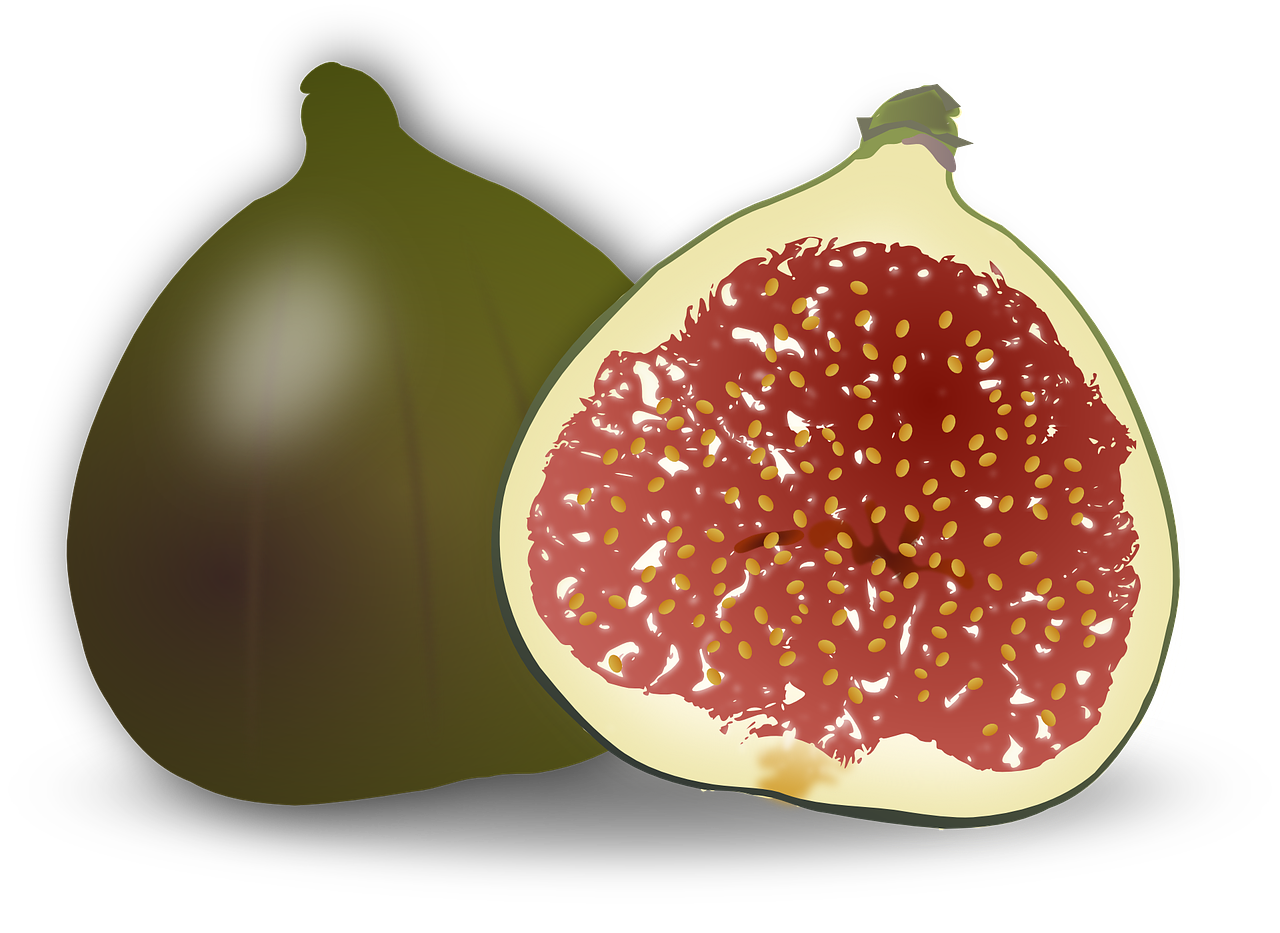
\includegraphics[width=0.6\textwidth,right]{ficus.png}
\caption{FICUS - Fluorescence Instrumentation Control Universal Software}\label{fig:fig0}
\end{minipage}
\end{figure}


	\clearpage
	
	        \section{Description}
        
       FICUS is a software designed to act on different levels: each level corresponds to a different subject who uses it and, consequently, a different choice of options available. In particular, three levels are available:
       \begin{itemize}
           \item \textbf{Detector Expert}: dedicated to detector and software developers, allows the maximum degree of variation of the available parameters and the display of screens useful for development and debugging;
           \item \textbf{Beamline Staff}: dedicated to the staff of the beamline, allows an intermediate degree of variation of the parameters for the setting and the measurement;
           \item \textbf{User}: dedicated to all possibile users of the beamline, allows a low degree of parameter variation but allows for data collection and pre-analysis.
       \end{itemize}
       
        \section{Applications}
        
        FICUS, after a preliminary selection of measurement parameters, performs the following tasks: data alignment of the cells, energy calibration, selection of the Region Of Interest (ROI). For example, during the measurement it is possible to obtain a spectrum in real time with some information such as FWMH and peak centroid (in ADC channels and in eV), count rate and dead time.
        
        \section{Features}
            \clearpage
	
\section{Guide for Detector Expert}
            %\subsection{Input}

Before starting any activity, please take a look at the \textbf{Safety warnings for using the SESAME-XAFS Detector System}, on page \pageref{accensione}, and the \textbf{Instructions for switching on/off}, respectively on page \pageref{accensione} and \pageref{spegnimento}.

This version of the software is recommended only for developers of the detector system in order to perform extensive testing and optimize performance.

\vspace{1cm}

After the launch of FICUS software, following the instructions recommended in this manual for switching on the detector system, the first window is the one shown in Fig. \ref{fig:fig1}.

        \begin{figure}[h]
        \centering
        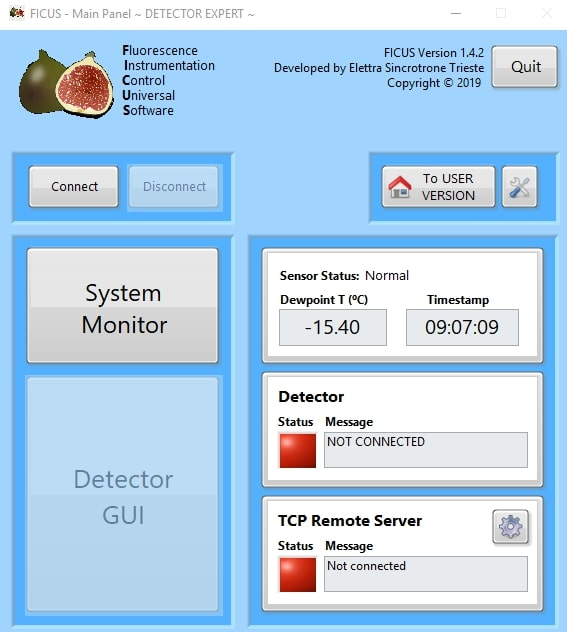
\includegraphics[scale=0.5]{Capture.jpg} \quad %width=0.7\textwidth
        \caption{The first window of FICUS software}\label{fig:fig1}
        \end{figure}
        

\begin{figure}[h]
\centering
\subfloat
{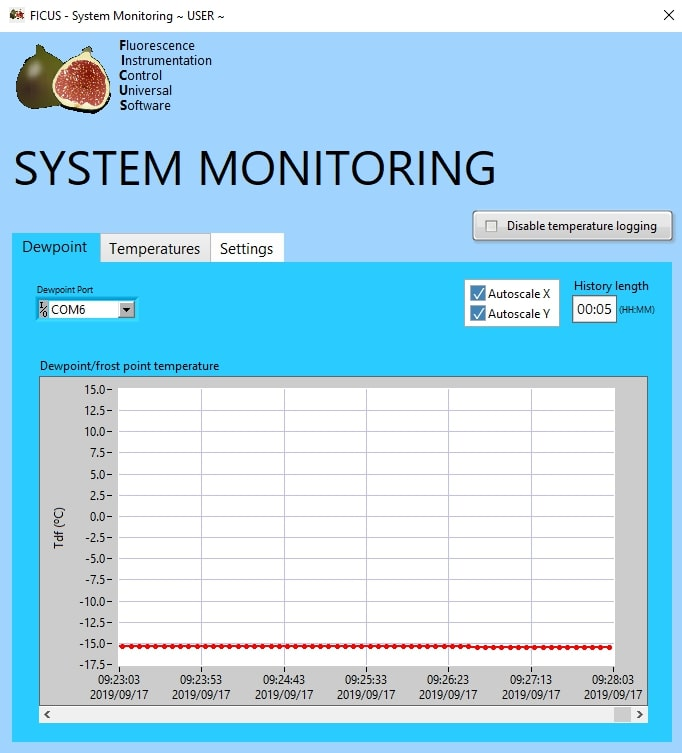
\includegraphics[width=.45\textwidth]{Capture15.jpg}} \quad
\subfloat
{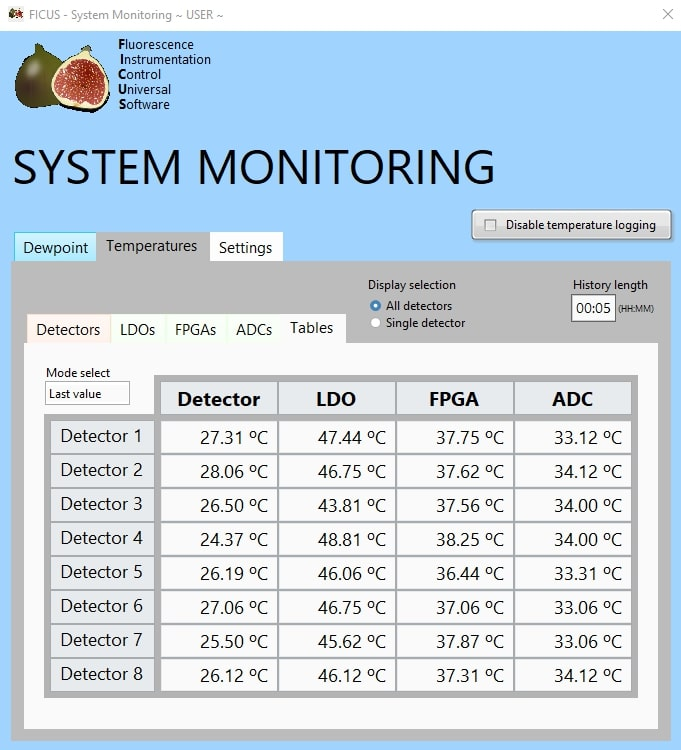
\includegraphics[width=.45\textwidth]{Capture19.jpg}} \\

\caption{(\textbf{a}) The log of the dew point temperature. (\textbf{b}) the table with all the last measured temperatures.}\label{fig:fig2}
\end{figure}

In the \textbf{System Monitor window} it is possible to see the dew point temperature of the system, the time, the status of the detectors and the status of the TCP Remote Server (red disconnected - green connected). 

After connect of the detector, it is also possible to click on \textit{System monitor} to know: 
\begin{itemize}
    \item the log of the dew point temperature [in Fig. \ref{fig:fig2} (a)]
    \item the log of the temperature of the strips [in Fig. \ref{fig:fig4} (a)]
    \item the log of the temperature of the LDOs [in Fig. \ref{fig:fig4} (b)]
    \item the log of the temperature of the FPGAs [in Fig. \ref{fig:fig4} (c)]
    \item the log of the temperature of the ADCs [in Fig. \ref{fig:fig4} (d)]
    \item the table with all the last measured temperatures [in Fig. \ref{fig:fig2} (b)]
    \item the setting for measuring temperatures [in Fig. \ref{fig:fig3}]
\end{itemize}

In the log it is possible to modify the time duration displayed and to set the extremes of the graph, or to set its auto setting.

\begin{figure}[h]
\centering
{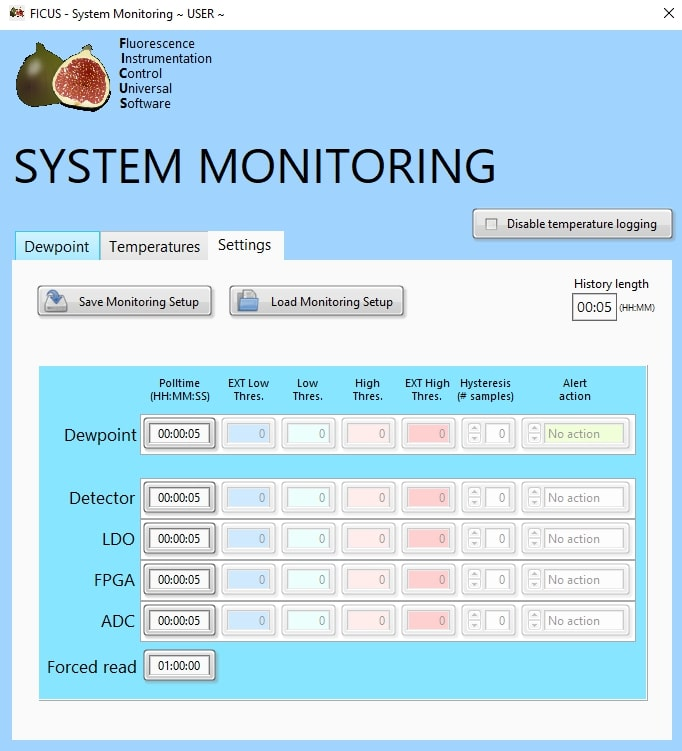
\includegraphics[width=.45\textwidth]{Capture20.jpg}} \quad
\caption{The setting for measuring temperatures.}\label{fig:fig3}
\end{figure}

\begin{figure}[h]
\centering
\subfloat
{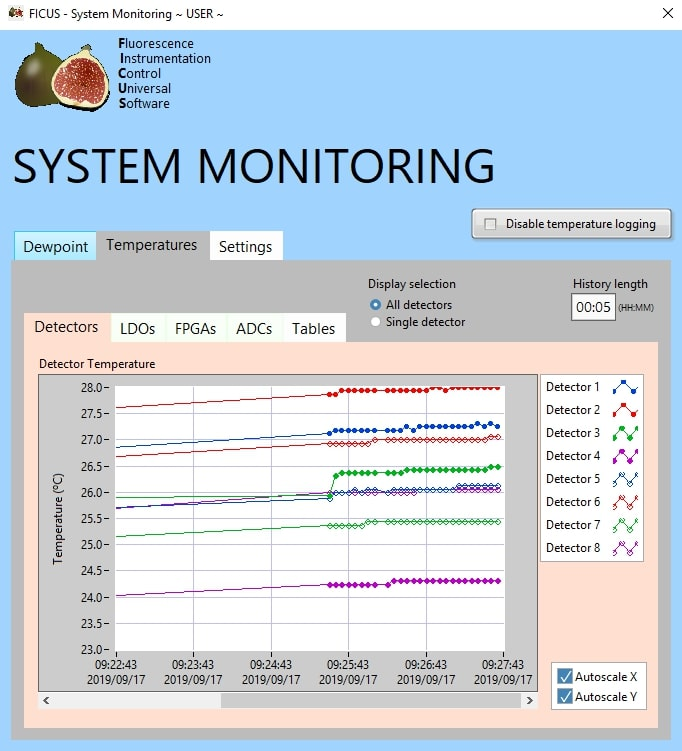
\includegraphics[width=.48\textwidth]{Capture14.jpg}} \quad
\subfloat
{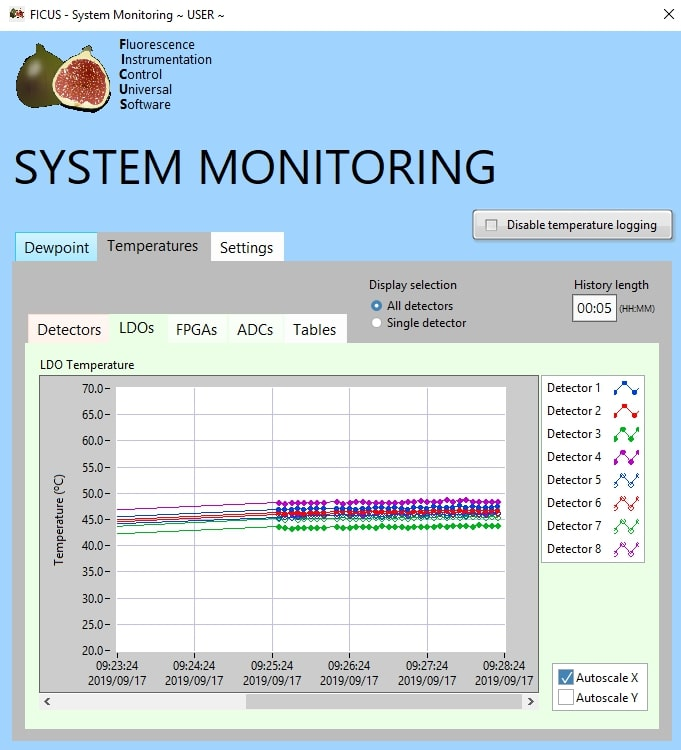
\includegraphics[width=.48\textwidth]{Capture16.jpg}} \\
\subfloat
{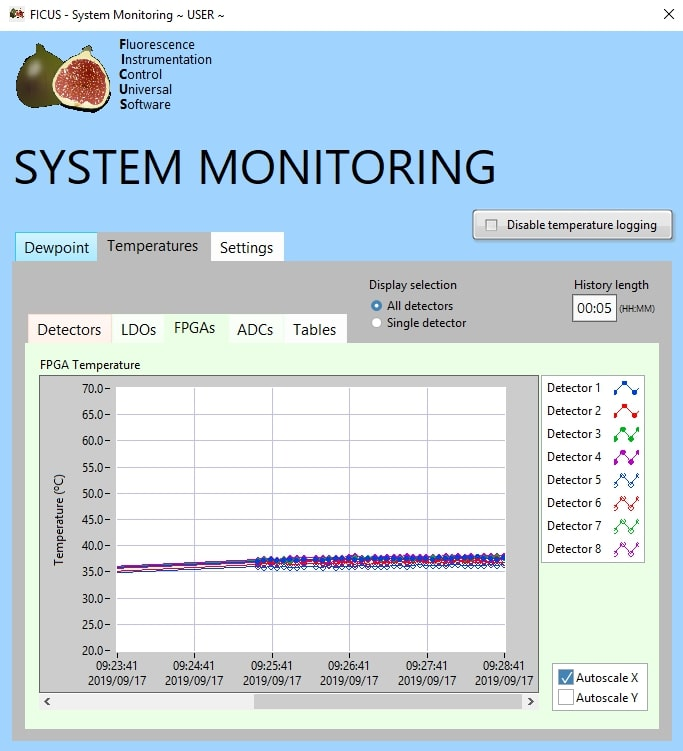
\includegraphics[width=.48\textwidth]{Capture17.jpg}} \quad
\subfloat
{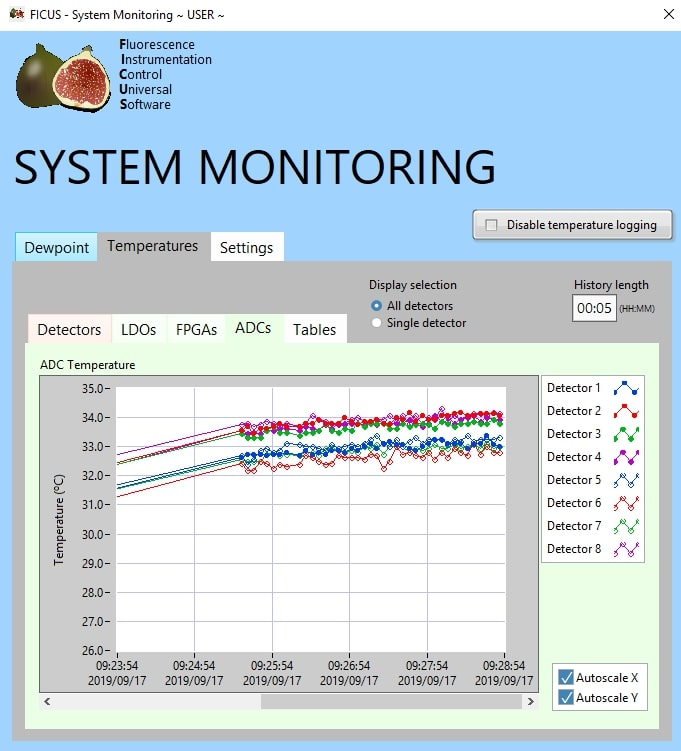
\includegraphics[width=.48\textwidth]{Capture18.jpg}} \\

\caption{In clockwise direction starting from the top left (\textbf{a}) The log of the temperature of the strips. (\textbf{b}) The log of the temperature of the LDOs. (\textbf{c}) The log of the temperature of the FPGAs. (\textbf{d}) the log of the temperature of the ASICs.}\label{fig:fig4}
\end{figure}
\clearpage 

To connect the detector system click on \textit{Connect} (in Fig. \ref{fig:fig1}). The connection window in Fig. \ref{fig:fig5} (a) appears. 
Click on \textit{Run TCP-IP and FPGA tests} and, if the test is successful, all the boxes will be colored green [Fig. \ref{fig:fig5} (b)] and you can proceed to the connection by clicking \textit{OK}.

\begin{figure}[h]
\centering
\subfloat
{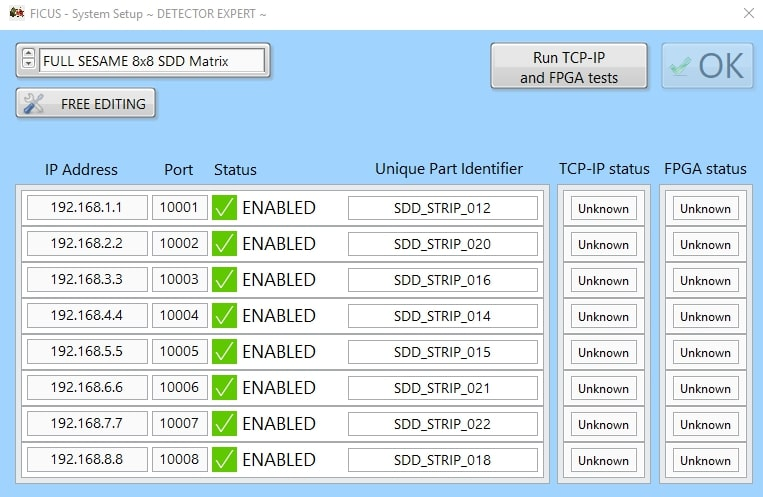
\includegraphics[scale=0.5]{Capture2.jpg}} \\
\subfloat
{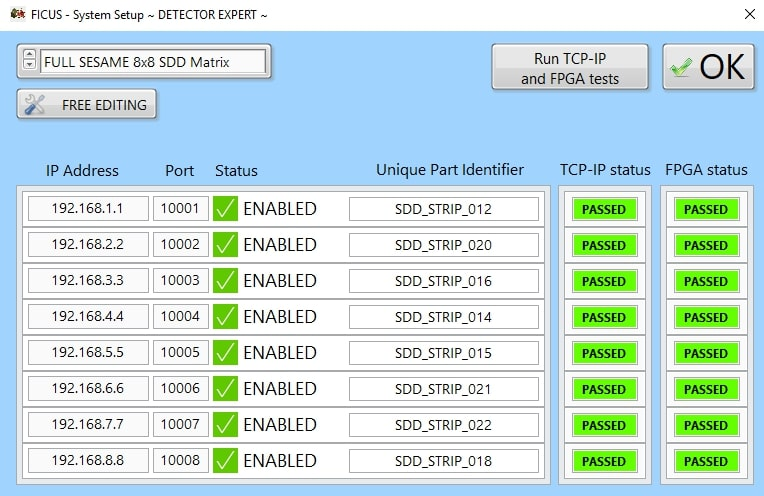
\includegraphics[scale=0.5]{Capture3.jpg}} \\
\caption{(\textbf{a}) The connection window - before connecting tests. (\textbf{b}) The connection window - after passing the connecting tests.}\label{fig:fig5}
\end{figure}

A message appears asking if you want to restore the previously used settings: press \textit{OK} to proceed or \textit{Cancel} to annul the setting restore [Fig. \ref{fig:fig6}]. It is possible to see that the status of the detector has changed to CONNECTED.

\begin{figure}[h]
\centering
{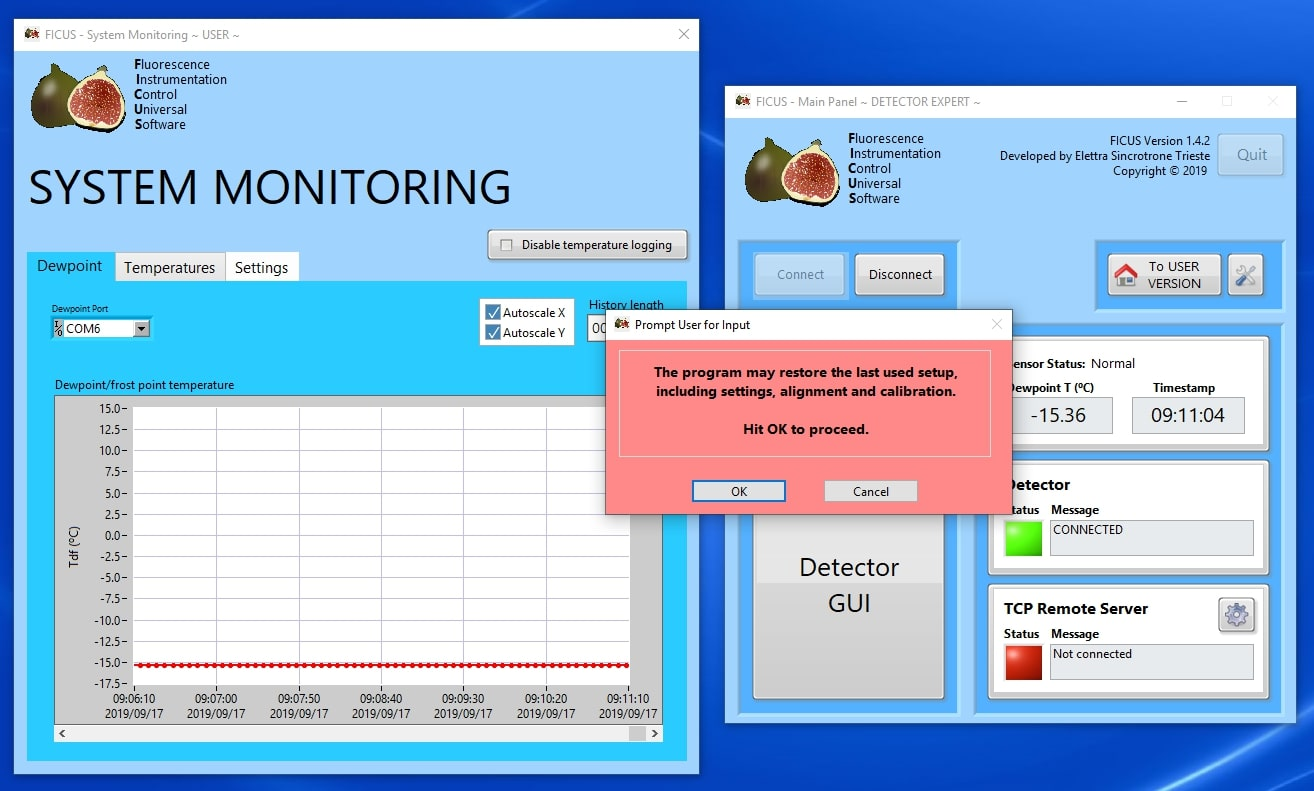
\includegraphics[width=.95\textwidth]{Capture4.jpg}} \quad
\caption{The final window for the connection.}\label{fig:fig6}
\end{figure}

\begin{figure}[h!]
\centering
{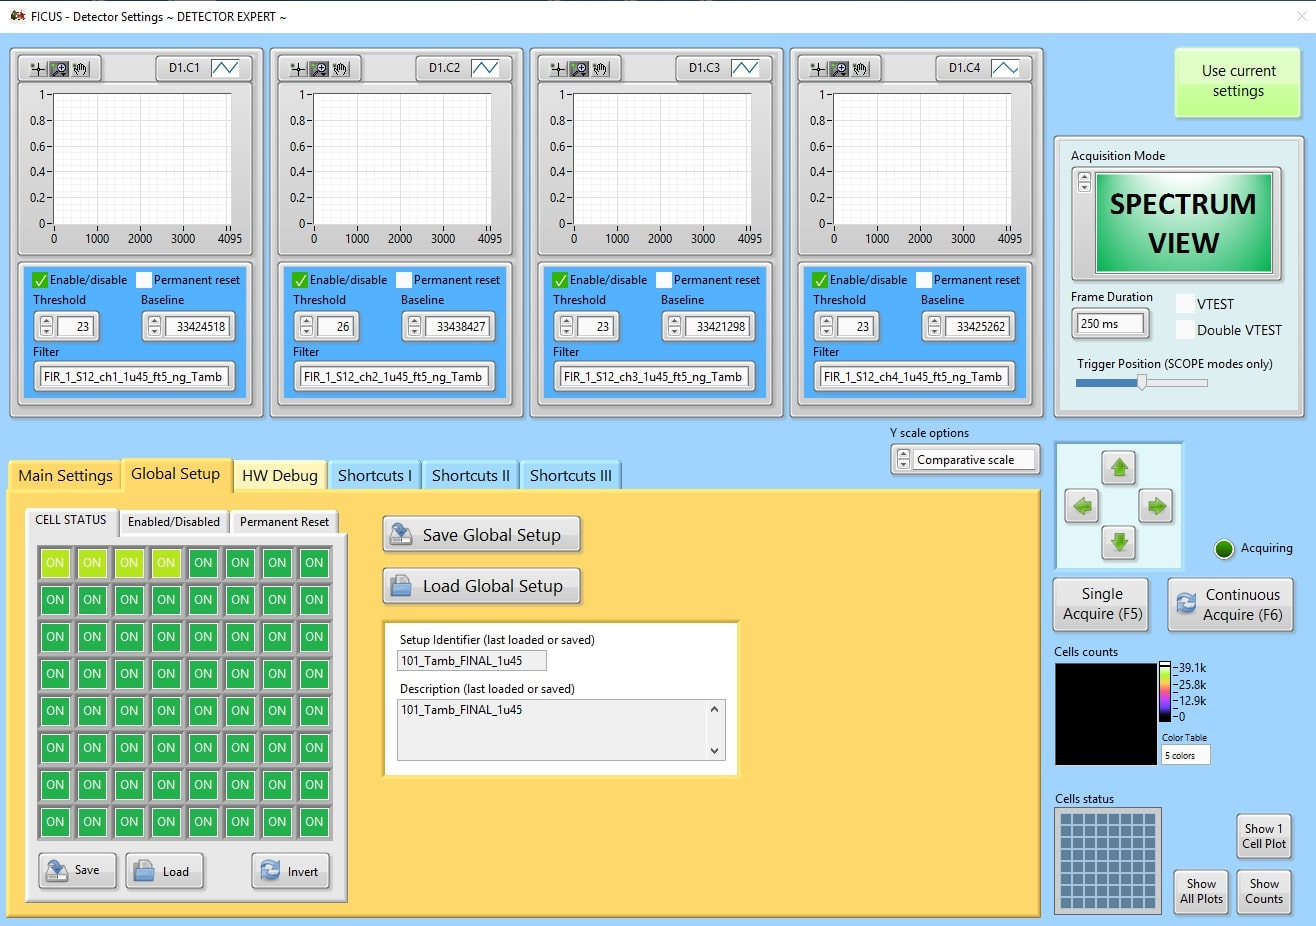
\includegraphics[width=.95\textwidth]{Capture8.jpg}} \quad
\caption{The first windows of the FICUS setting (with Global Setup).}\label{fig:fig7}
\end{figure}

The first window of the \textbf{FICUS settings} opens, in \textit{Spectrum View} [Fig. \ref{fig:fig7}]. Here, at the top from the left you can see the signals of the individual channels: 4 at a time (those highlighted in light green in the panel at the bottom left), and you can change which ones to select by clicking on the green arrows in the center on the right. In in the panel at the bottom left, in addition to the \textit{Cell Status}, it is also possible to display the map of the \textit{Enabled/Disabled} channels [Fig. \ref{fig:fig7bis} (a)], and the map of the channels in \textit{Permanent Reset} [Fig. \ref{fig:fig7bis} (b)]. Within each box in the upper part, it is possible \textit{Enable/disable} the channel, put the channel in \textit{Permanent reset}, and manually set the \textit{Threshold}, \textit{Baseline} and \textit{Filter}. \\
In the upper right corner, it is possible to enable and disable the test signals (\textit{VTEST} and \textit{Double VTEST}) and to select the \textit{Frame Duration} (among the values: 5 ms, 7.5 ms, 10 ms, 25 ms, 50 ms, 75 ms, 100 ms, 250 ms, 500 ms, 750 ms, 1 s, 2.5 s, 5 s, 7.5 s, 10 s, and External Gate).\\
In the central part on the right there are buttons to activate the measurement: \textit{Single Acquire (F5)} and \textit{Continuous Acquire (F6)}, and a green dot indicating the acquisition in progress. \\
In the lower right part of the window there are: a graph with the Cells counts represented (with the graduated scale of colors next to it), one with the Cells status visible (where in grey it is an unavailable channel, in green an active and counting channel, in red an inactive and with error channel, in black a disabled channel, and in dark green an active and with no counts channel, placed in permanent reset). There are also three buttons (\textit{Show 1 Cell Plot}, \textit{Show All Plots}, \textit{Show Counts}), which allow you to view respectively the detail of the signal of a channel [Fig. \ref{fig:fig9} (a)], the contemporary graph of all 64 channels [Fig. \ref{fig:fig8}] and the counts of 64 channels [Fig. \ref{fig:fig9} (b)]. In this graphs it is possible to change X and Y scale of the histograms.

\begin{figure}[h]
\centering
\subfloat
{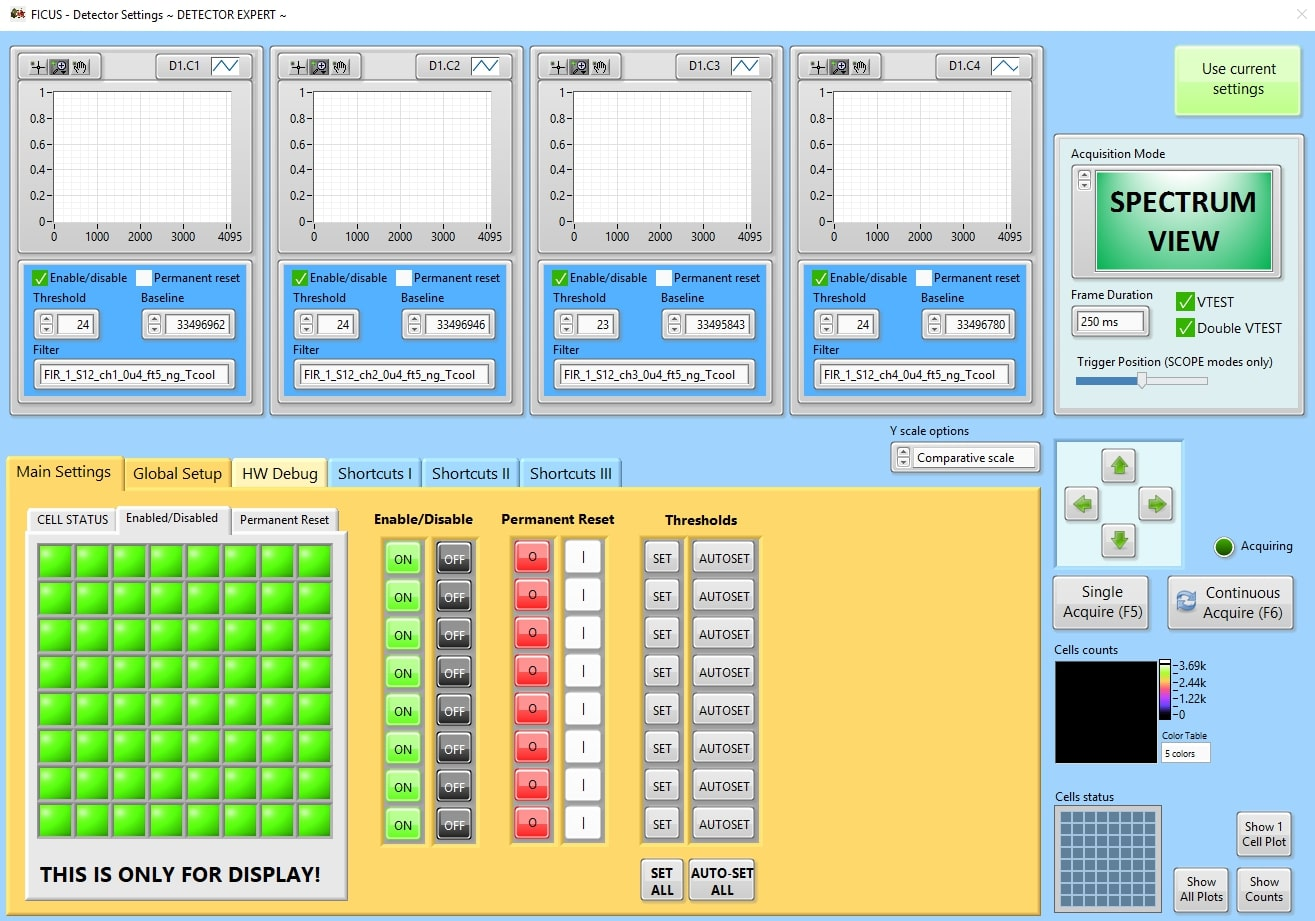
\includegraphics[width=.48\textwidth]{Capture60.jpg}} \quad
\subfloat
{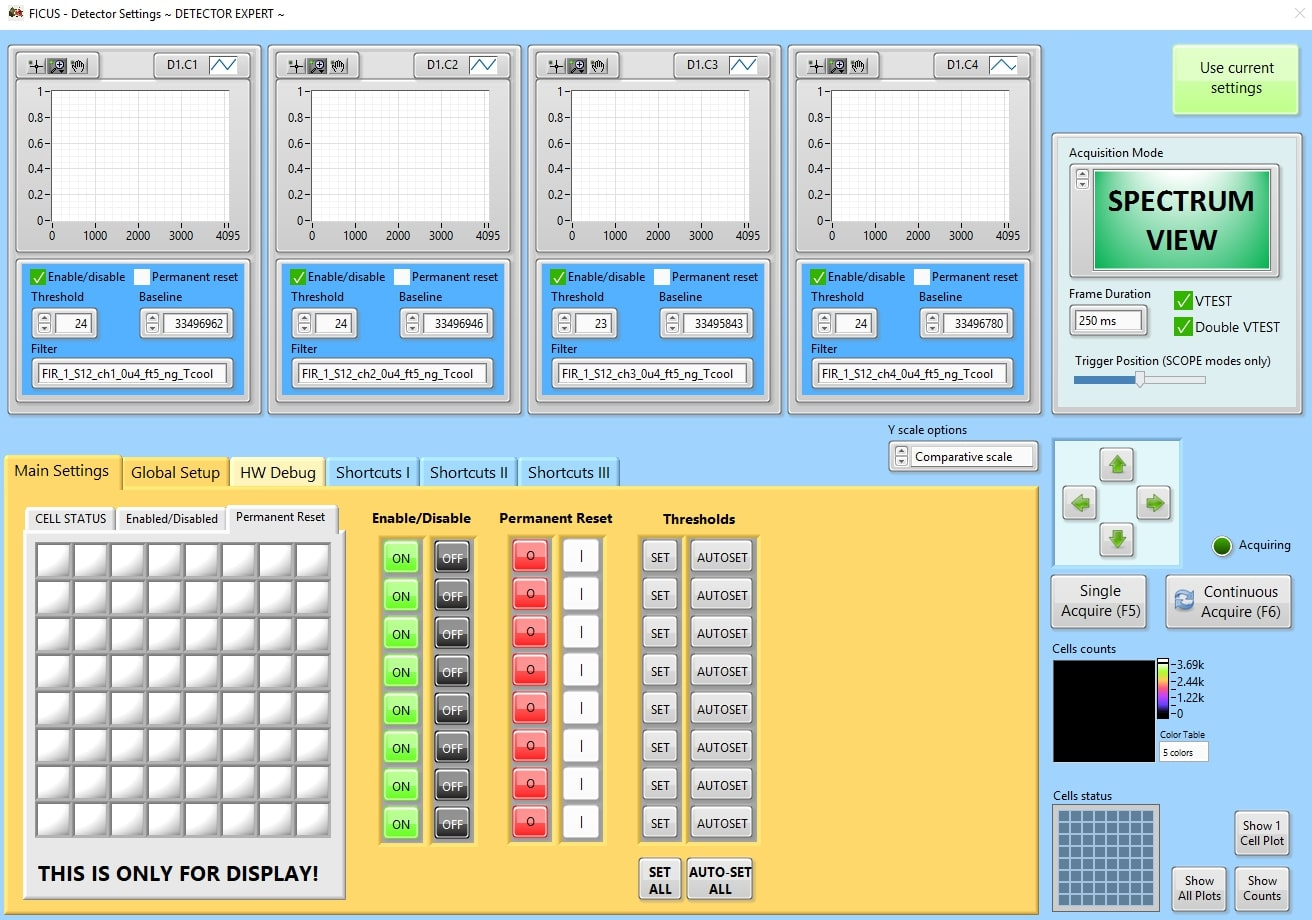
\includegraphics[width=.48\textwidth]{Capture61.jpg}} \\
\caption{The windows of the FICUS setting, in Main Setting (\textbf{a}) Enabled/Disabled, and (\textbf{b}) Permanent Reset channels.}\label{fig:fig7bis}
\end{figure}

\begin{figure}[h]
\centering
{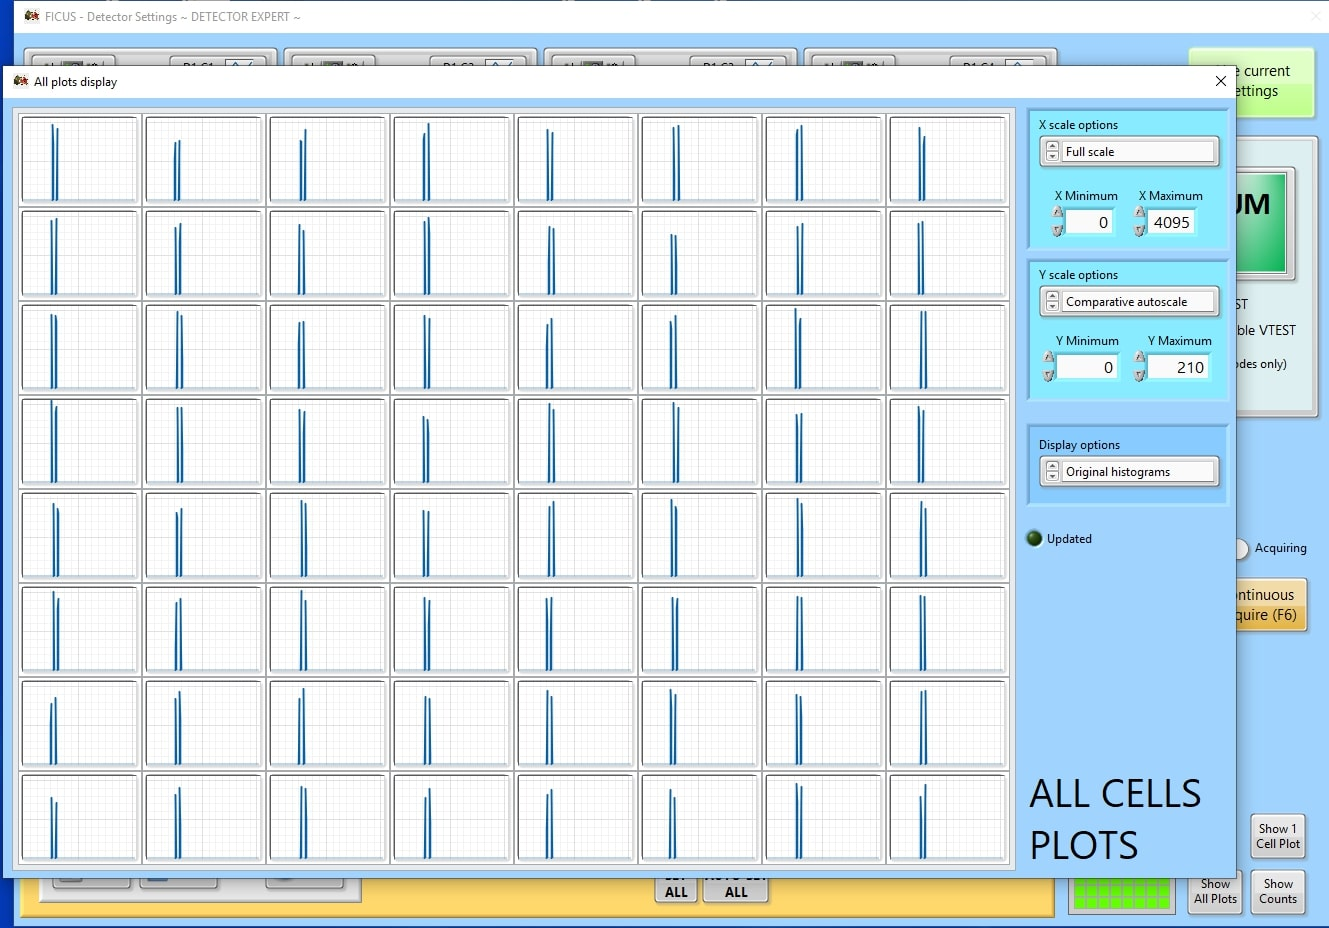
\includegraphics[width=.80\textwidth]{Capture21.jpg}} \quad
\caption{The windows of the FICUS with Show All Plots, with VTEST and Double VTEST enabled.}\label{fig:fig8}
\end{figure}

\begin{figure}[h]
\centering
\subfloat
{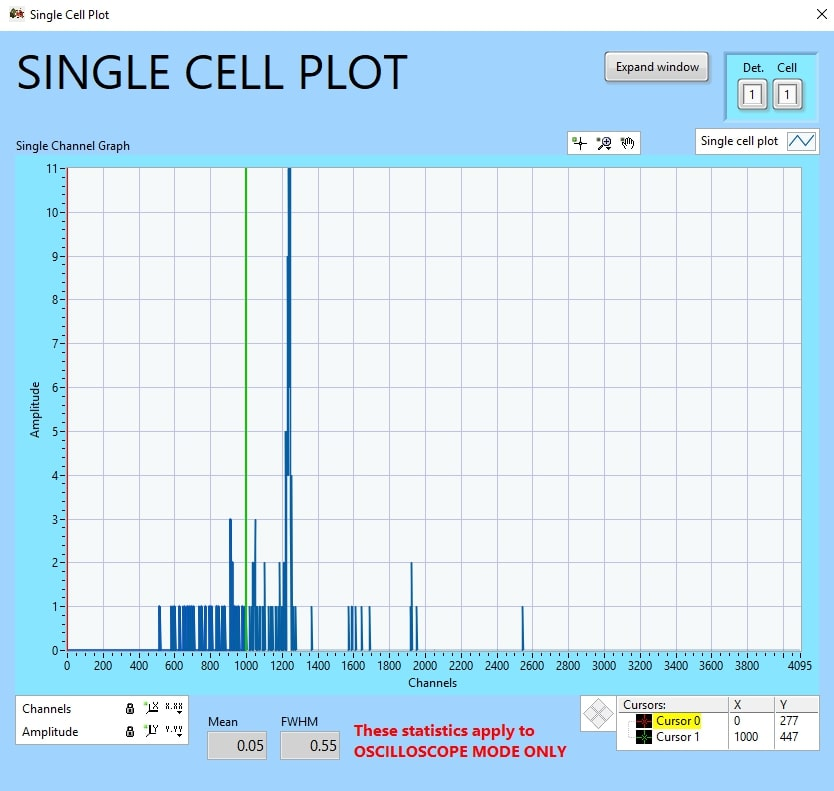
\includegraphics[width=.35\textwidth]{Capture43.jpg}} \quad
\subfloat
{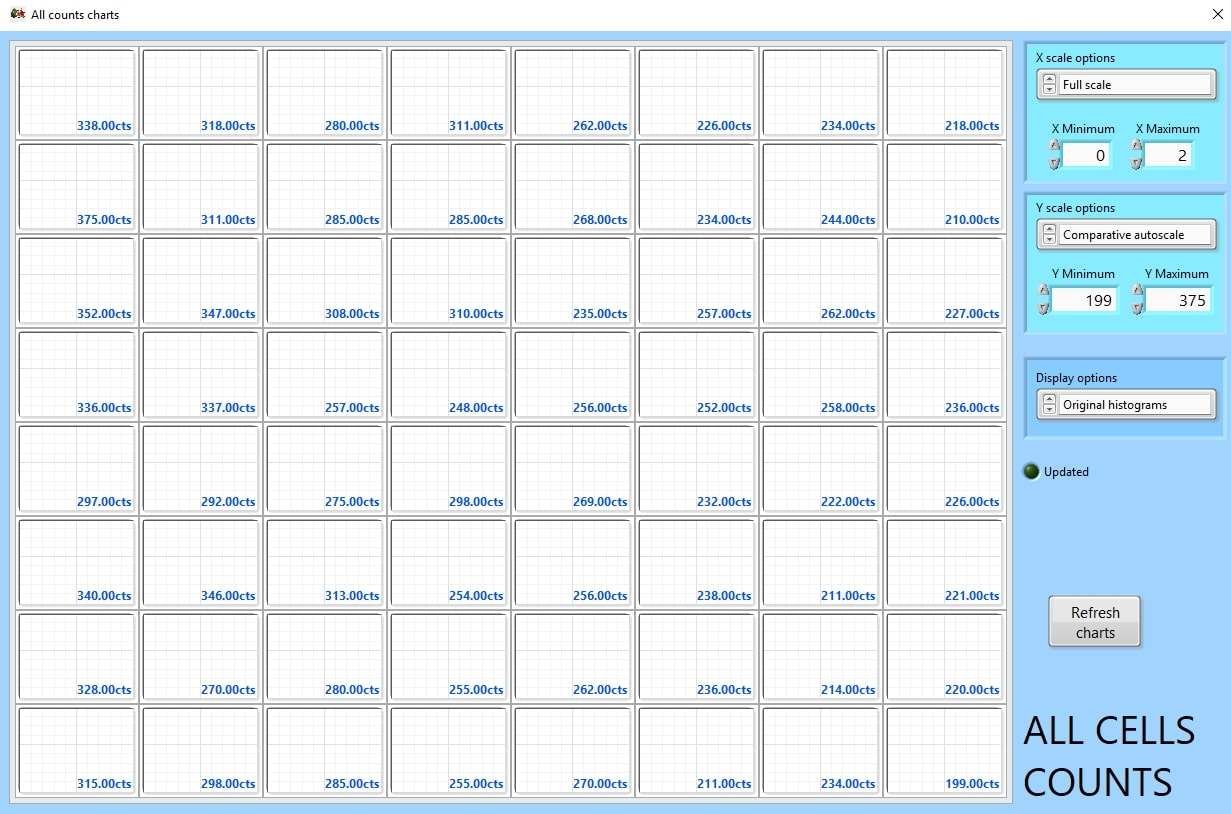
\includegraphics[width=.55\textwidth]{Capture42.jpg}} \\
\caption{The windows of the FICUS with (\textbf{a}) Show 1 Cell Plot, and (\textbf{b}) Show Counts.}\label{fig:fig9}
\end{figure}

In the central part of the window, there is an additional menu that modifies the central part of the window by enabling further possible adjustments. \\
In \textit{Global Setup} there is the possibility to save (assigning a name and notes) the current settings, with \textit{Save Global Setup}, or to open settings already set and saved, with \textit{Load Global Setup}. if you select the latter option in particular, a further window opens in which it is possible to choose from the 8 pre-set global setups: four different possible filter lengths (0.4, 0.7, 1, and 1.45 $\mu$s) at two possible cell temperatures (at room temperature, Tamb, and with cooled cells with voltage on the Peltier cells, Tcool) [Fig. \ref{fig:fig10} (a)]. After selecting the one you want, just click on \textit{OK, load this setup}, and \textit{Yes} at the next confirmation window that opens, as in Fig. \ref{fig:fig10} (b).

\begin{figure}[h]
\centering
\subfloat
{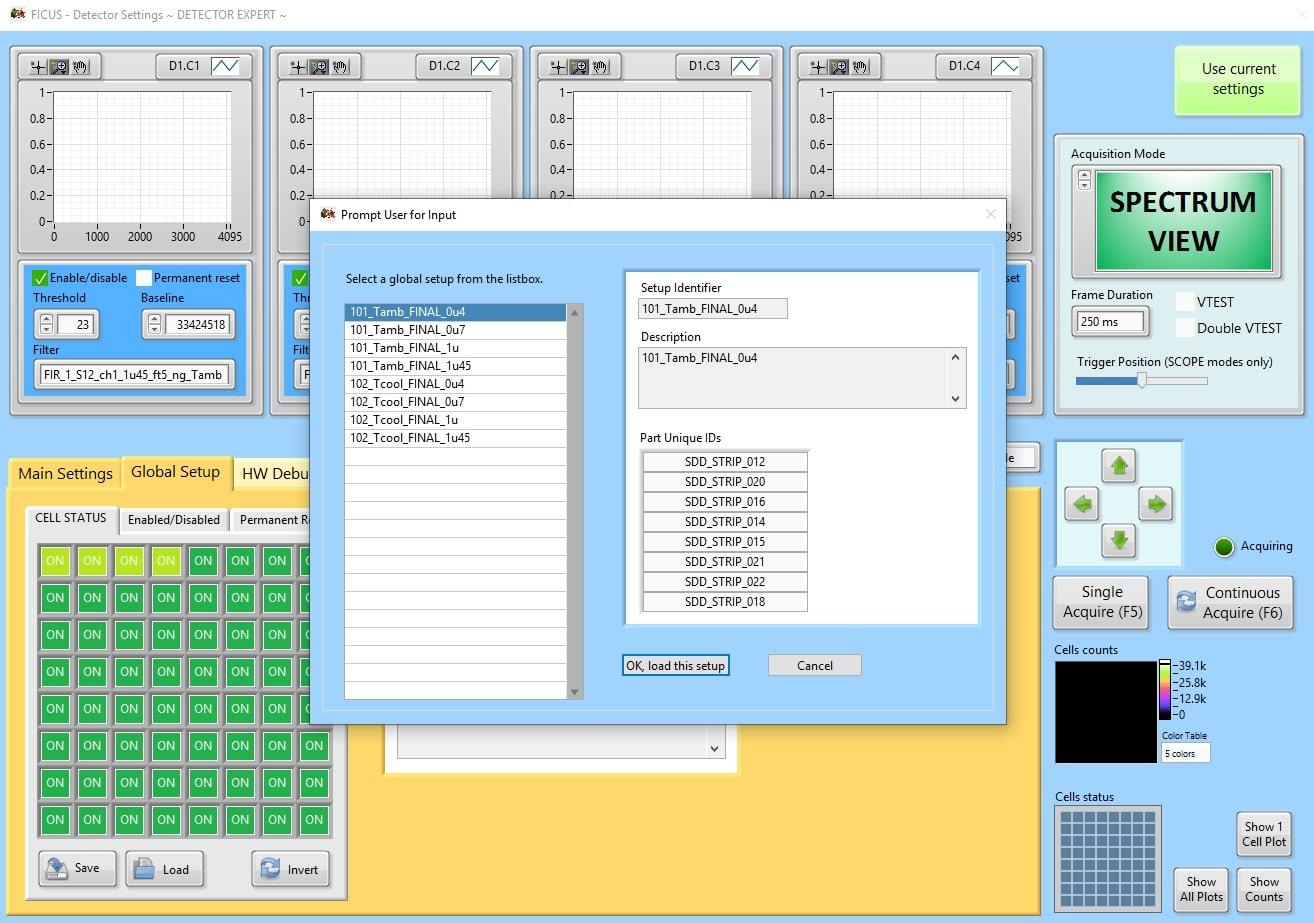
\includegraphics[width=.85\textwidth]{Capture6.jpg}} \\
\subfloat
{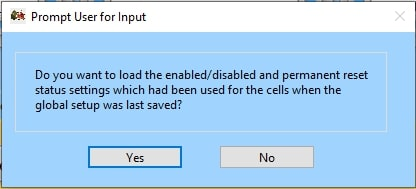
\includegraphics[width=.30\textwidth]{Capture7.jpg}} 
\caption{(\textbf{a}) The windows in which it is possible to choose from the 8 pre-set global setups, and (\textbf{b}) the confirmation window.}\label{fig:fig10}
\end{figure}

In \textit{Main Setting} [Fig. \ref{fig:fig11}] it is possible to \textit{Enable/Disable} all the channels of one strip, put all the channels of one strip in \textit{Permanent Reset}, and \textit{Set} the \textit{Threshold}, for each strip or for all strips at the same time, manually or in \textit{Autoset}.

\begin{figure}[h]
\centering
{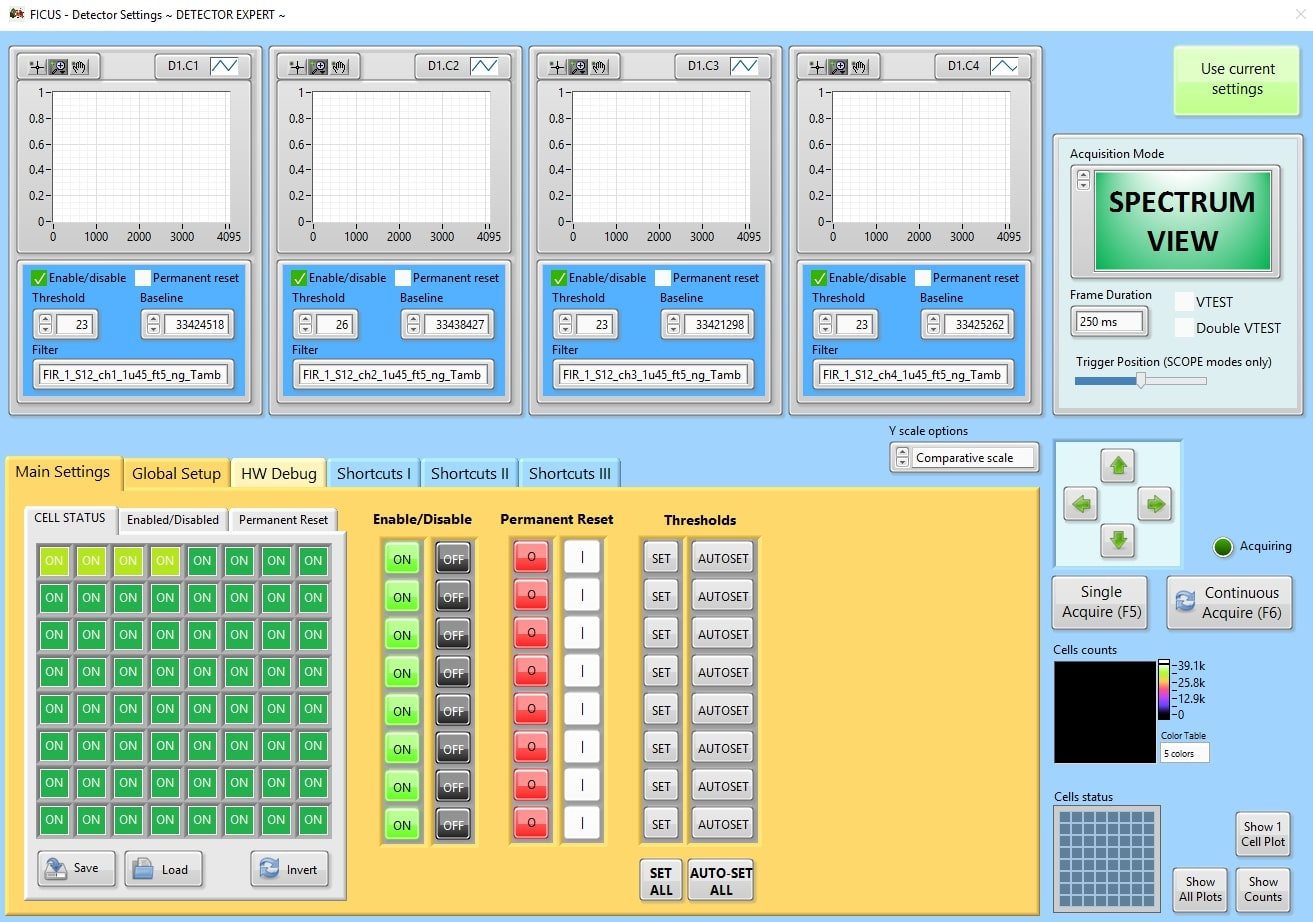
\includegraphics[width=.85\textwidth]{Capture9.jpg}} \quad
\caption{The windows of the FICUS setting (with Main Setting) in Spectrum View.}\label{fig:fig11}
\end{figure}

In \textit{HW Debug} [Fig. \ref{fig:fig12}] it is possible to see the \textit{PART IDs} of every strips of the detector system and to \textit{TEST} and \textit{RESET}, if it necessary, for each strip or for all strips at the same time, the FPGAs.

\begin{figure}[h]
\centering
{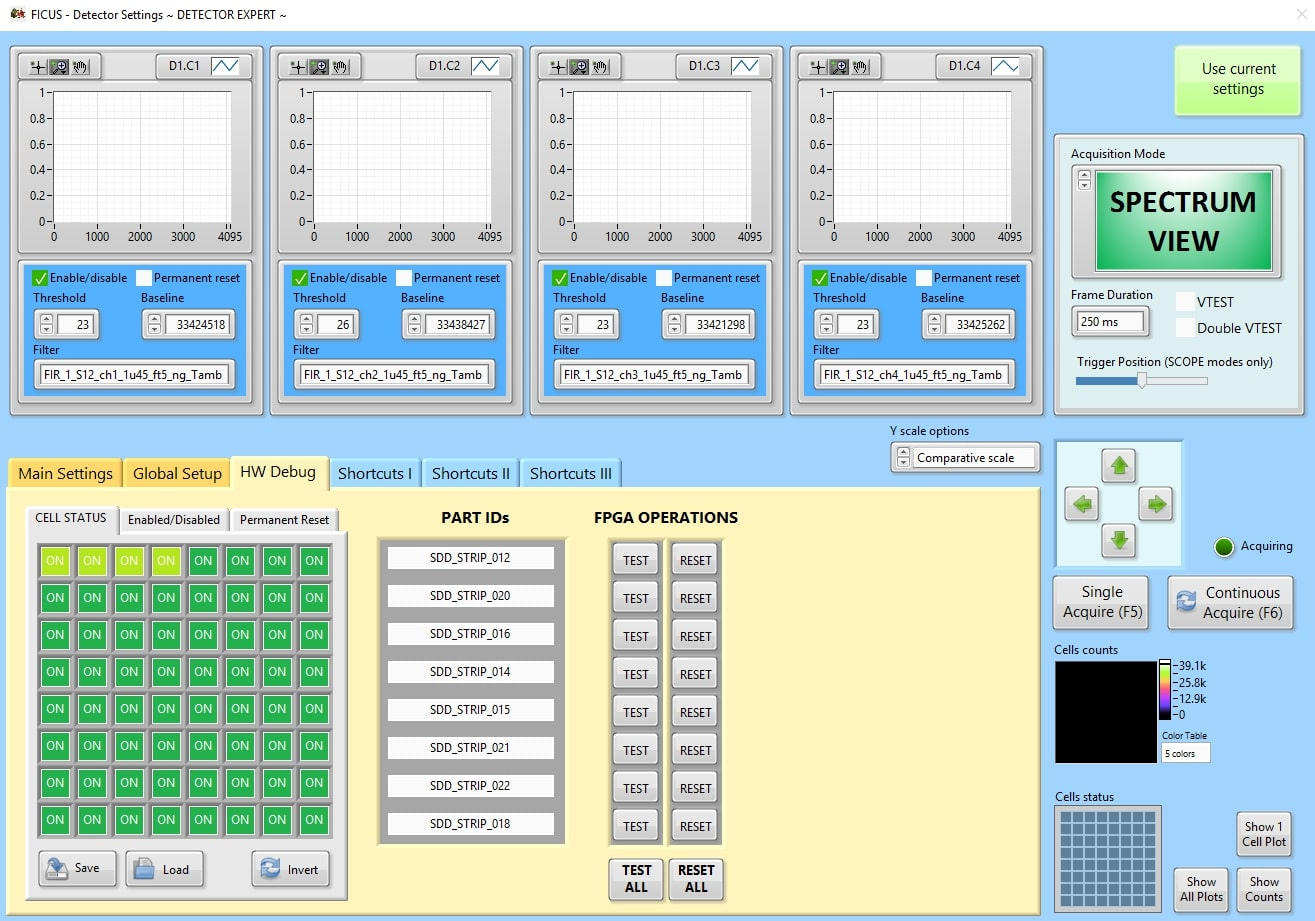
\includegraphics[width=.85\textwidth]{Capture10.jpg}} \quad
\caption{The windows of the FICUS setting (with HW Debug).}\label{fig:fig12}
\end{figure}

In \textit{Shortcuts I} [Fig. \ref{fig:fig13}] it is visible the \textit{MANAGE SETTING}. Here it is possible to \textit{STORE}, \textit{RECALL} and \textit{APPLY} the current setting, for each strip or for all strips at the same time.

\begin{figure}[h]
\centering
{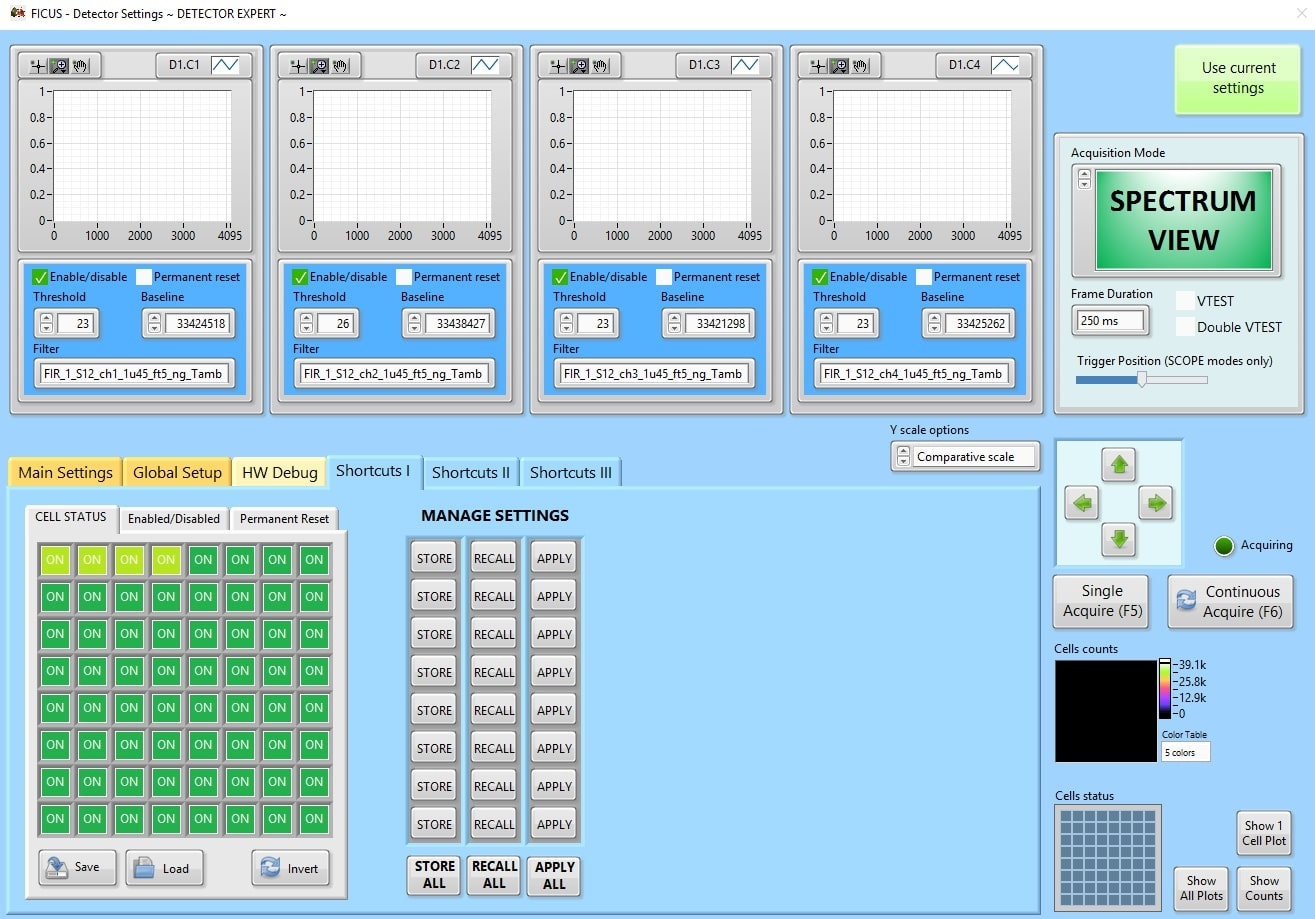
\includegraphics[width=.85\textwidth]{Capture11.jpg}} \quad
\caption{The windows of the FICUS setting (with Shortcuts I).}\label{fig:fig13} 
\end{figure}

In \textit{Shortcuts II} [Fig. \ref{fig:fig14}] there are settings for the \textit{Baselines} and for the \textit{filters}; in particular, it is possible to \textit{SET} the Baselines manually or in \textit{Autoset} (based on the parameters provided in the I box), and upload the Filters, for each strip or for all strips at the same time. 

\begin{figure}[h]
\centering
{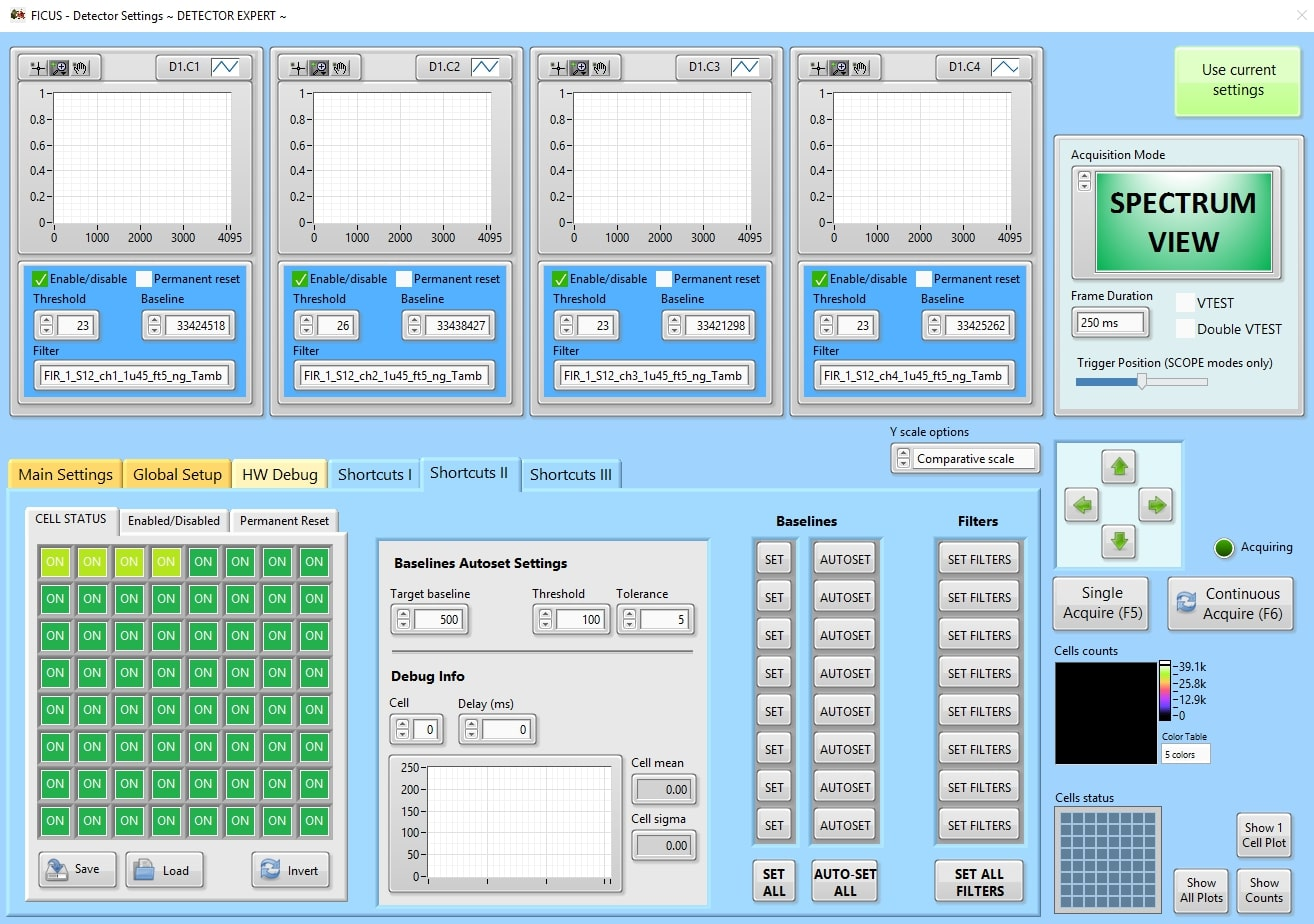
\includegraphics[width=.85\textwidth]{Capture12.jpg}} \quad
\caption{The windows of the FICUS setting (with Shortcuts II).}\label{fig:fig14}
\end{figure}

In \textit{Shortcuts I\textit{\textit{}}} [Fig. \ref{fig:fig15}] it is possible to know the \textit{ADC status} and the \textit{RTD Table Filenames} for every strip. It is also possible to set the \textit{Filter Binary Cut} and the \textit{Reset Parameters}: \textit{Trigger} (FIX/AUTO), \textit{Frequency}, \textit{Width}, and \textit{Delay}.

\begin{figure}[h]
\centering
{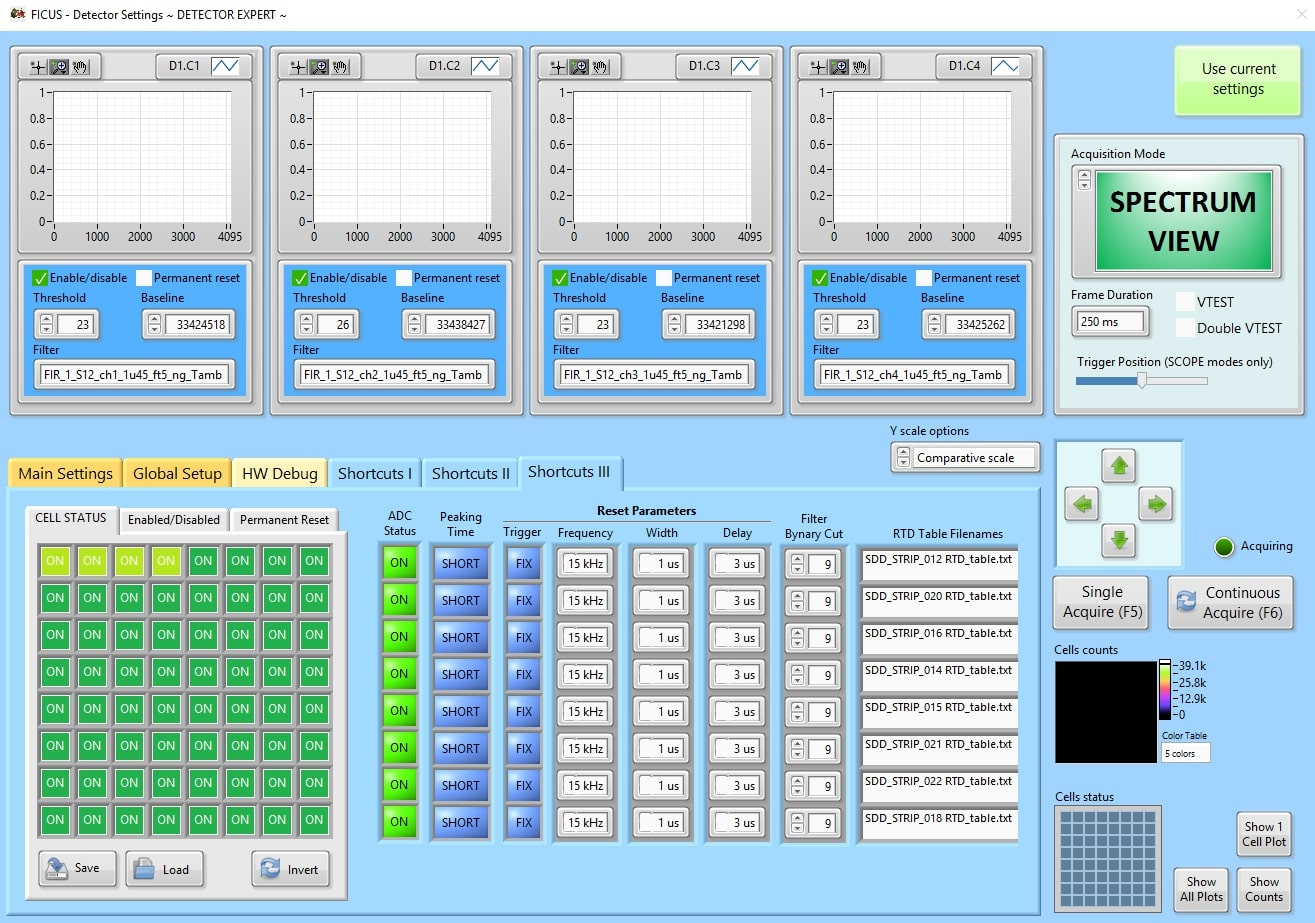
\includegraphics[width=.85\textwidth]{Capture13.jpg}} \quad
\caption{The windows of the FICUS setting (with Shortcuts III).}\label{fig:fig15}
\end{figure}


As it can be seen in Fig. \ref{fig:fig16}, it is possible to change acquisition mode and switch from \textit{Spectrum View} (used for normal acquisition) to \textit{Scope View (RAW Data)} (used for RAW data acquisition), \textit{Scope View (Filtered Data)} (used for acquisition of filtered RAW data), and \textit{Scope View (Long Time)}.

\begin{figure}[h]
\centering
{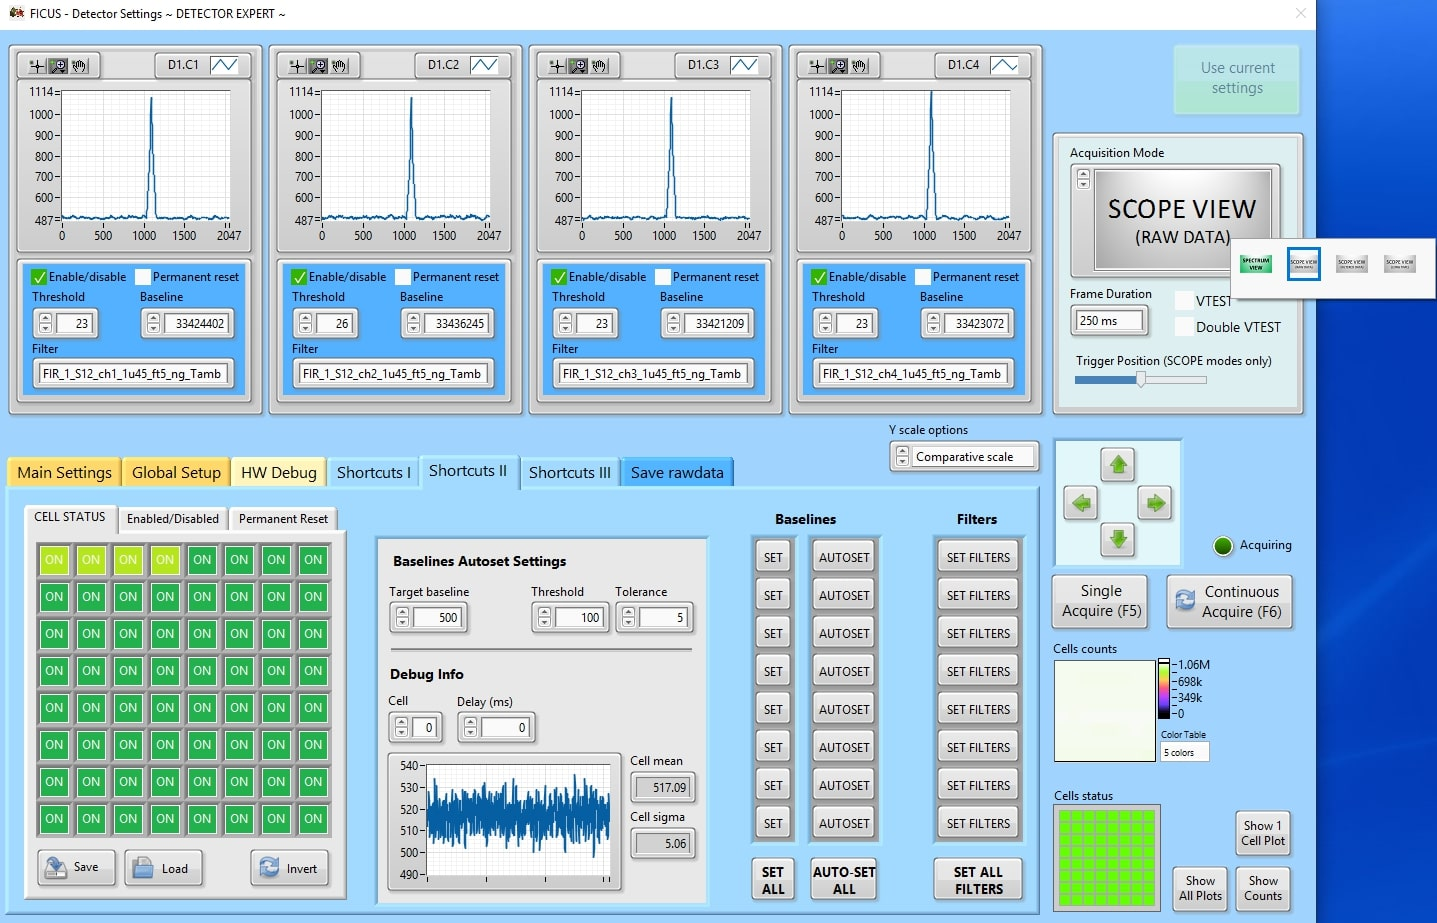
\includegraphics[width=.95\textwidth]{Capture22.jpg}} \quad
\caption{The windows of the FICUS setting (menu of Acquisition Mode).}\label{fig:fig16}
\end{figure}

When switching to \textit{Scope View (RAW Data)} Acquisition Mode, the \textit{Save rawdata} field appears in the middle of the page, through which you can set the duration of the raw acquisition, the file name and the save folder; during the acquisition, the Elapsed time after the end is indicated [Fig. \ref{fig:fig17}].

\begin{figure}[h]
\centering
{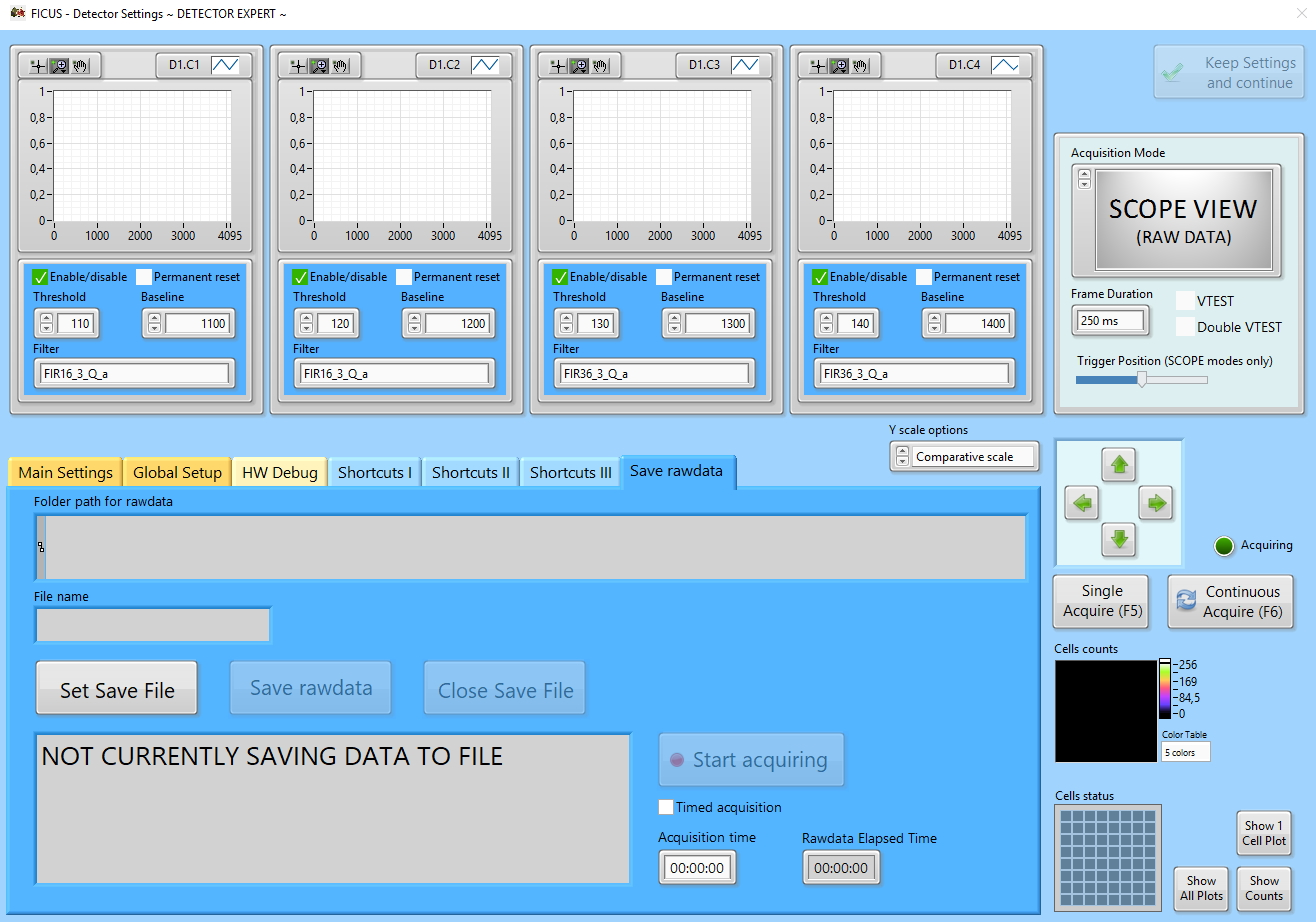
\includegraphics[width=.85\textwidth]{Cattura64.jpg}} \quad
\caption{The windows of the FICUS setting (Scope View - rawdata).}\label{fig:fig17}
\end{figure}

When the settings are all set it is possible switch to acquisition window: to do so you have to return to the \textit{Spectrum View Acquisition Mode} and click on the green button at the top right \textit{Use current setting}.
The FICUS acquisition window opens, which appears as in Fig. \ref{fig:fig18}. To return to the settings just click on the \textit{HW Setting} button.

\clearpage

\begin{figure}[h]
\centering
{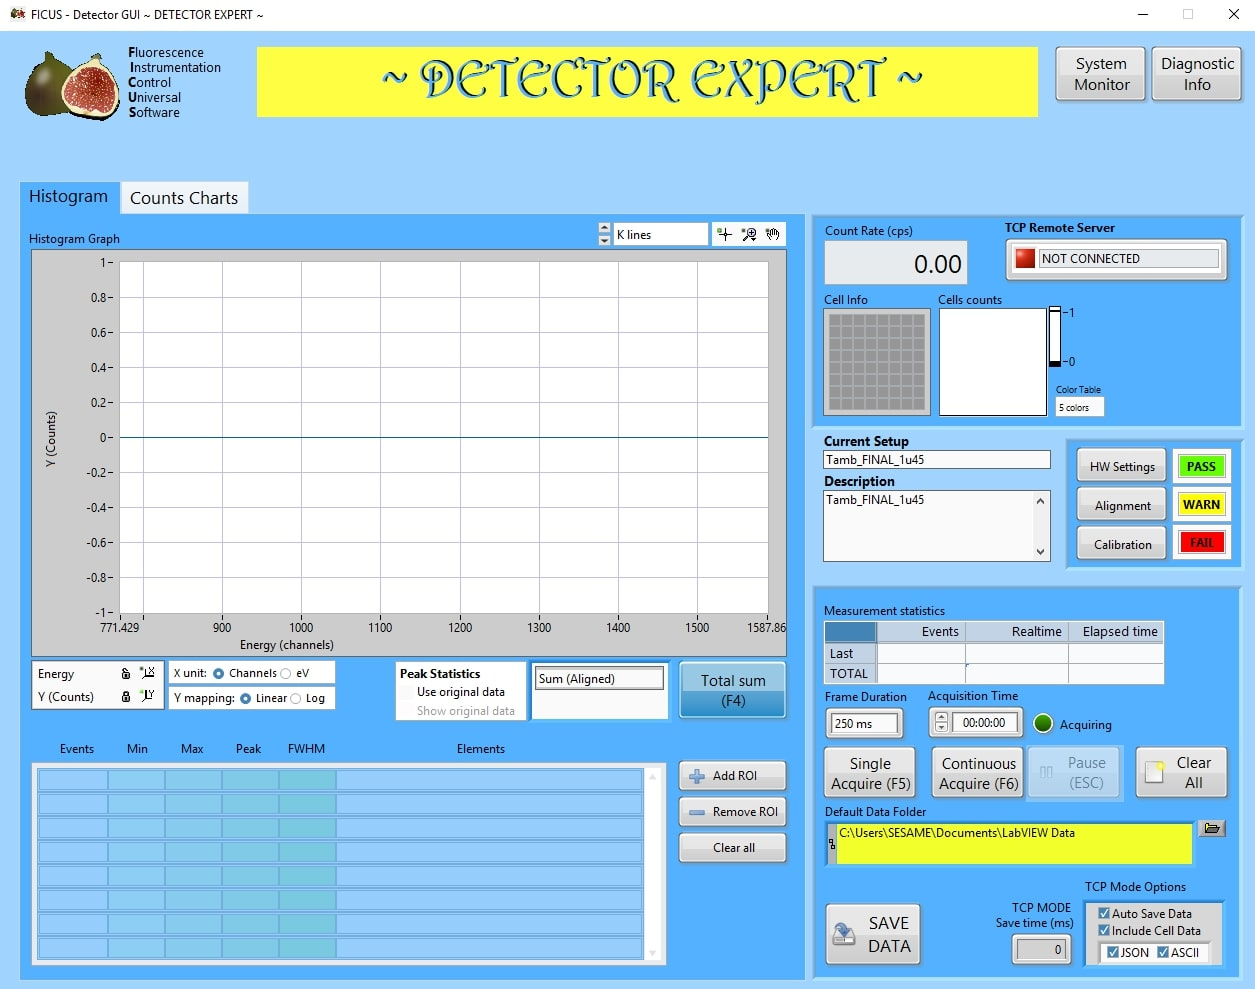
\includegraphics[width=.9\textwidth]{Capture33.jpg}} \quad
\caption{The windows of the FICUS acquisition (Histogram), before alignment and starting the measurement.}\label{fig:fig18}
\end{figure}

The \textbf{FICUS acquisition window}, by clicking on the corresponding buttons in the upper right corner, it is possible to open the window of \textit{System Monitor}, as shown in Figs. \ref{fig:fig2} - \ref{fig:fig3} - \ref{fig:fig4}, and the \textit{Diagnostic Info}, as shown in Figs. \ref{fig:fig27}. The windows of Diagnostic Info are used to verify the correct functioning of the detector through detailed information regarding the status [Figs. \ref{fig:fig27} (a)], counts [Figs. \ref{fig:fig27} (b)], dead time [Figs. \ref{fig:fig27} (c)], and pile-up [Figs. \ref{fig:fig27} (d)] of all channels. From these windows (using the buttons in the upper part is \textit{Show 1 Cell Plot} in Figs. \ref{fig:fig9} (a), \textit{Show Counts} [Figs. \ref{fig:fig9} (b)], and \textit{Show All Plots} [Figs. \ref{fig:fig28}]) it is possible to have detailed information of the signal collected.


\begin{figure}[h]
\centering
\subfloat
{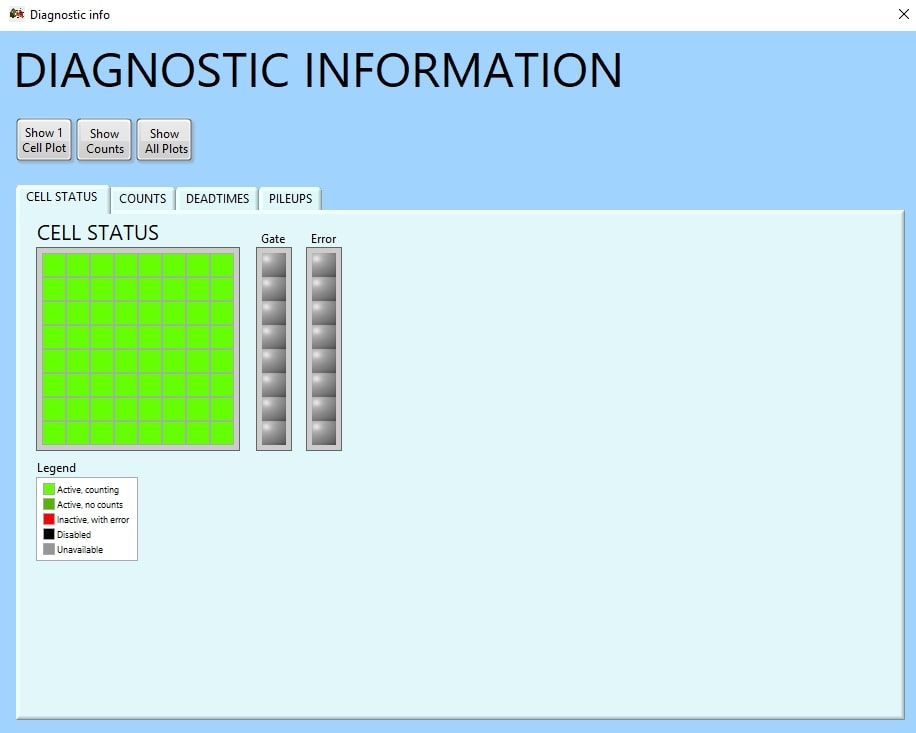
\includegraphics[width=.48\textwidth]{Capture37.jpg}} \quad
\subfloat
{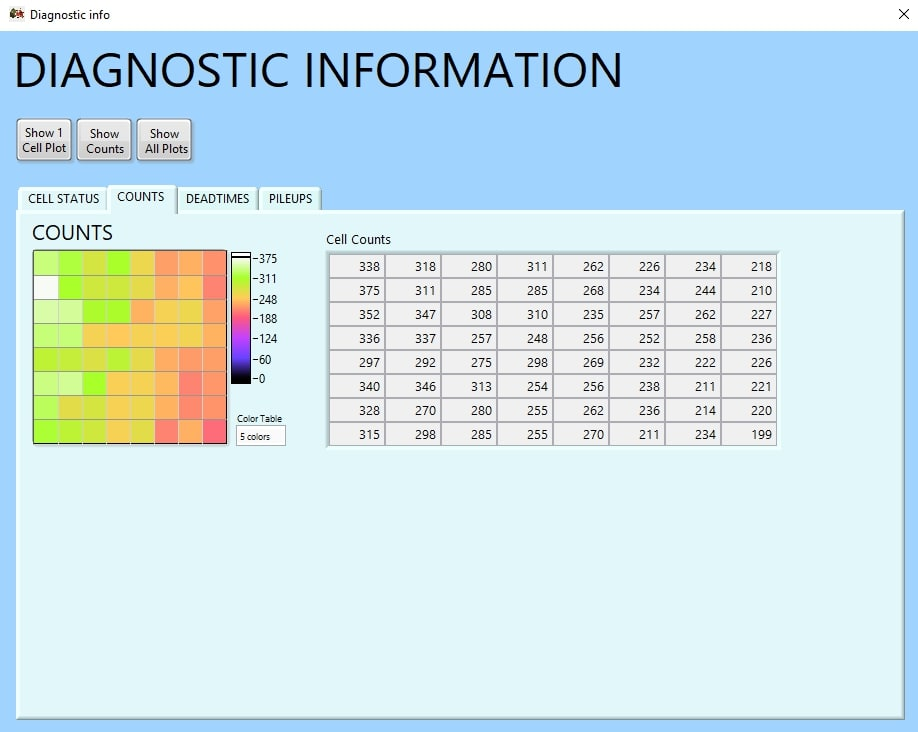
\includegraphics[width=.48\textwidth]{Capture38.jpg}} \\
\subfloat
{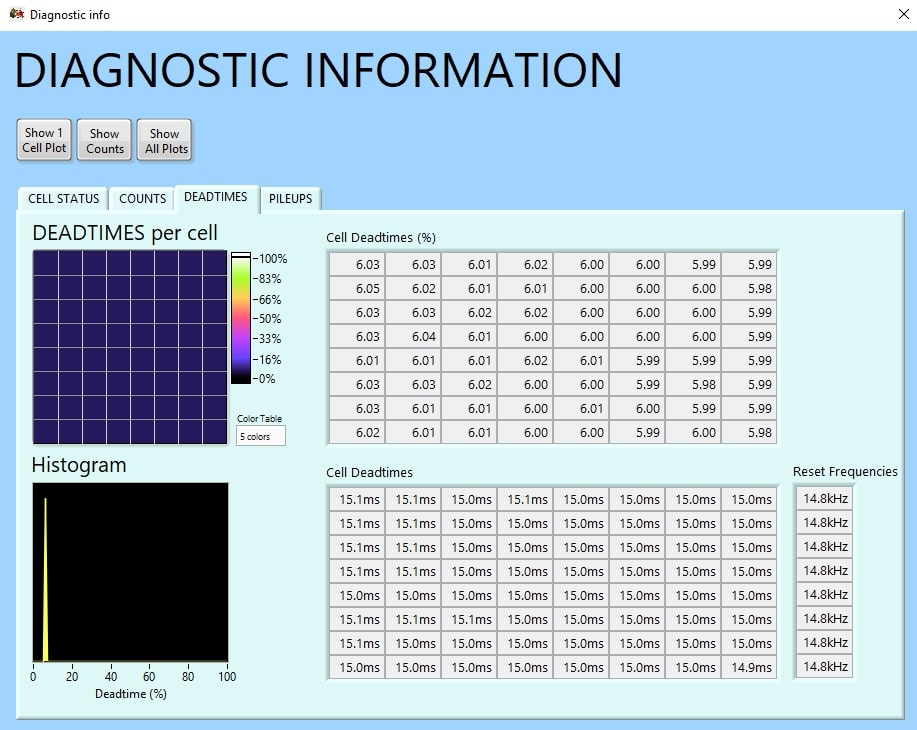
\includegraphics[width=.48\textwidth]{Capture39.jpg}} \quad
\subfloat
{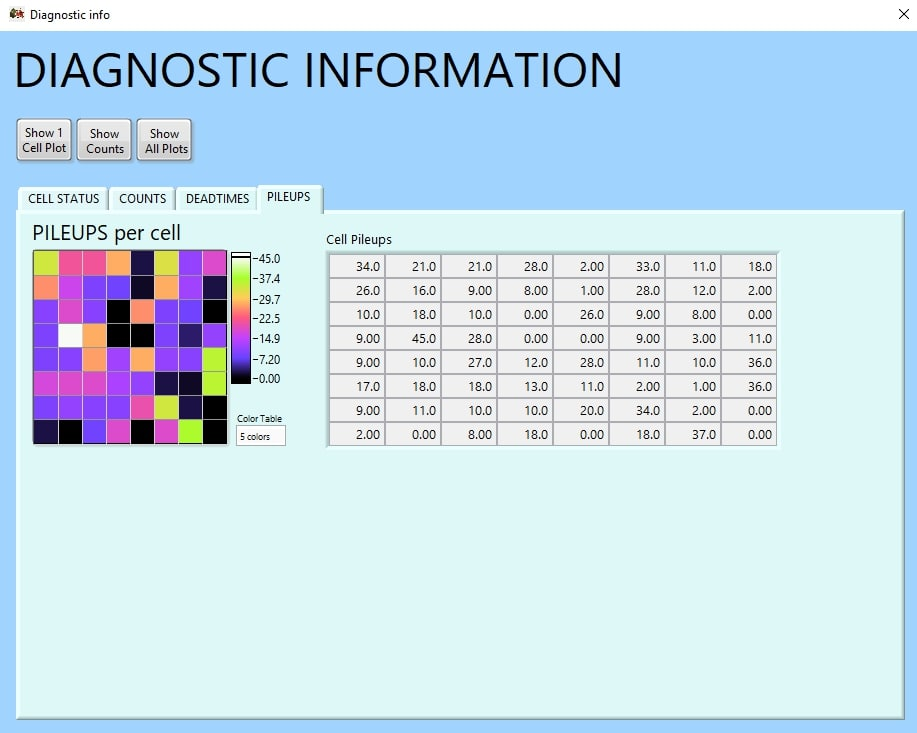
\includegraphics[width=.48\textwidth]{Capture40.jpg}} \\
\caption{The windows of the FICUS Diagnostic Information (\textbf{a}) Cell Status, (\textbf{b}) Counts, (\textbf{c}) Deadtimes, (\textbf{d}) Pileups.}\label{fig:fig27}
\end{figure}


\begin{figure}[h]
\centering
{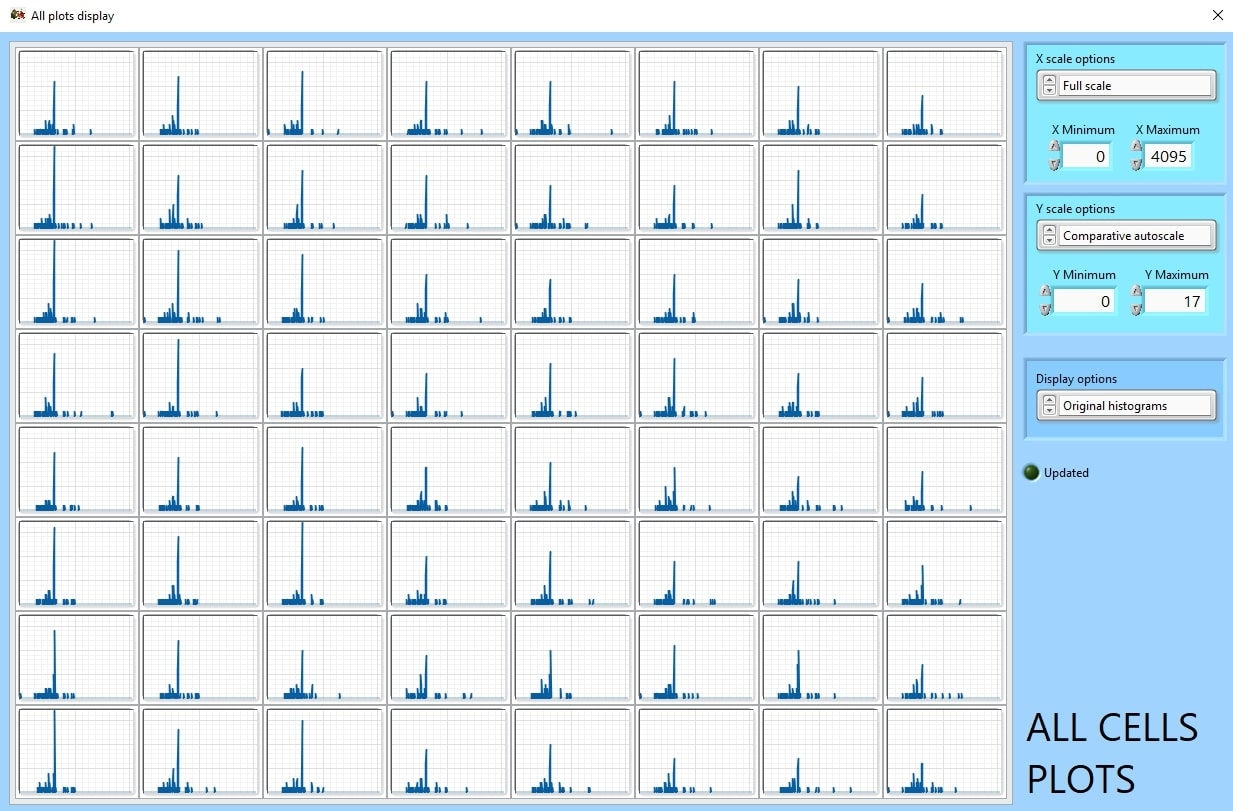
\includegraphics[width=.82\textwidth]{Capture41.jpg}} \quad
\caption{The windows of the FICUS with Show All Plot.}\label{fig:fig28}
\end{figure}


\clearpage

On the right of the FICUS acquisition window it is possible to know the count rate of the acquisition (in counts/s), an overview of information on the functioning of the cells and on the counts cell by cell. In addition, the TCP Remote Server connection information is also visible. Under this box, are visible the name and description of the Global Setup in use, and next to them there are buttons to open the \textit{HW Setting}, \textit{Alignment} and \textit{Calibration} windows; next to each of them there is an indicator that has three possible aspects: \textit{PASS} in green (which means that that setting was made), \textit{WARNING} in yellow (which means that that setting has been done previously, but something has been changed since then and you may need to redo the setting), and \textit{FAIL} in red (which means that that setting has never been done before and you need to do the setting).

Clicking on \textit{Alignment} opens the window dedicated to it. The top and right parts of the \textbf{FICUS Alignment window} are always the same; through the mid-page menu it is possible to change the bottom-left part of the window.
In the Alignment window, from the Figs. \ref{fig:fig19} to the Fig. \ref{fig:fig22}, in the alignment window there is the possibility to load a pre-saved alignment (by clicking on \textit{Load from file...}), to align the channels starting from a new acquisition (by starting the acquisition with the \textit{Start/Stop acquiring} button) or to align the channels starting from saved data (by using the \textit{Original data, load from file...} top left button).

On the right side, starting from the top, it is possible to select manually manually, indicating the detector (\textit{Det.}) and cell (\textit{Cell}), the channel with respect to which to align the others or select the box \textit{Autoselect Cell} for automatic alignment (in which the software, using the chosen criterion, chooses the most appropriate box with respect to which to align the channels); in the graph, on which it is impossible to act, the channels with respect to which the system is aligning are displayed.
To align is necessary to choose the \textit{Alignment Parameters}: \textit{Peak Reject} (selects only the peaks with the minimum required height compared to the highest), \textit{Peak Width} (selects only the peaks with minimum required width), and the \textit{number of Peak to Use}.  
Below it is possible, after starting the acquisition or loading the data and selecting the alignment parameters, to calculate the parameters (\textit{Recalc parameters}, selecting \textit{Live recalc}) and apply them, clicking on \textit{Apply parameters}.

After starting the acquisition (click on \textit{Flush} to restart from zero), at the top of the window it is possible to see the histogram (of all channels or only some channels) of the accumulated signal (it is possible change manually the ends of the axes or you can zoom by clicking on the magnifying glass symbol); two markers can be used to delimit the ends of the signal on which to make the alignment. An indicator is provided to indicate that the acquisition is in progress.

In the middle of the Alignment windows there is a menu that allows you to change the information displayed:
\begin{itemize}
    \item \textit{Alignment Results} - allows to display a preview of the aligned signal sum [in Fig. \ref{fig:fig21} (a)]
    \item \textit{\# Peaks} - allows to see how many peaks of the signal of each channel correspond to the set parameters, and therefore are useful for the alignment. When all channels have the same number of peaks (which is also the one chosen in \textit{# of Peak to Use}), the green light will light up. [in Fig. \ref{fig:fig20}]
    \item \textit{Centers} - allows you to see the position of the centroid, it is possible to select the peak [in Fig. \ref{fig:fig21} (b)]
    \item \textit{Counts} - allows to see the counts of the cell [in Fig. \ref{fig:fig21} (c)]
    \item \textit{Max Value} - allows to see the maximum counts of the cell [in Fig. \ref{fig:fig22} (a)]
    \item \textit{Delta} - maximum [peak centers] - minimum [peak centers] NB CHIARIRE CON LUIGI, the total of all channels and the total for each strip are also displayed [in Fig. \ref{fig:fig22} (b)]
    \item \textit{FWHM} -  allows to see the FWHM of the cell, it is possible to select the peak, and the total of all channels and the total for each strip are also displayed [in Fig. \ref{fig:fig19}]  
    \item \textit{Norm. FWHM Quad (\%)} - NB CHIARIRE CON LUIGI, the total of all channels and the total for each strip are also displayed [in Fig. \ref{fig:fig22} (c)]
\end{itemize}

\begin{figure}[h]
\centering
{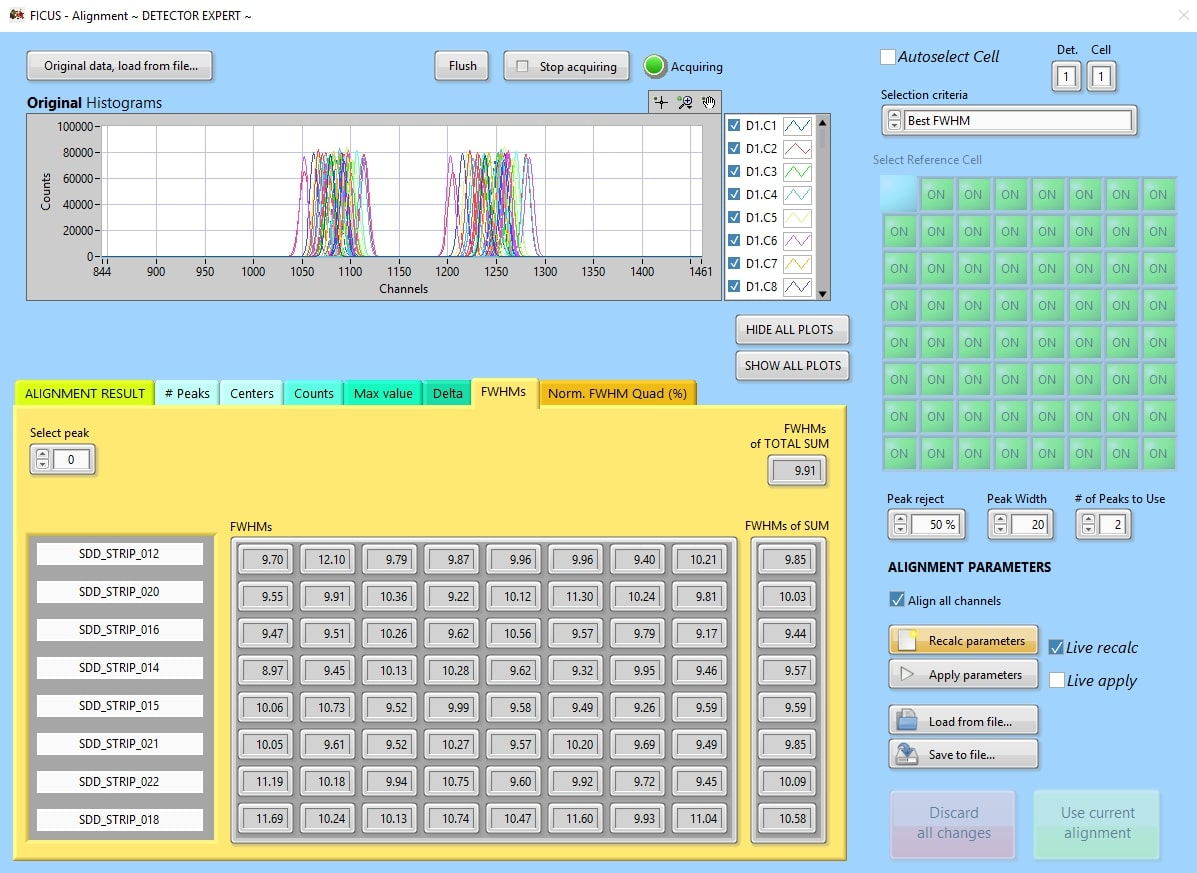
\includegraphics[width=.7\textwidth]{Capture29.jpg}} \quad
\caption{The windows of the FICUS Alignment (FWHM).}\label{fig:fig19}
\end{figure}

\begin{figure}[h]
\centering
{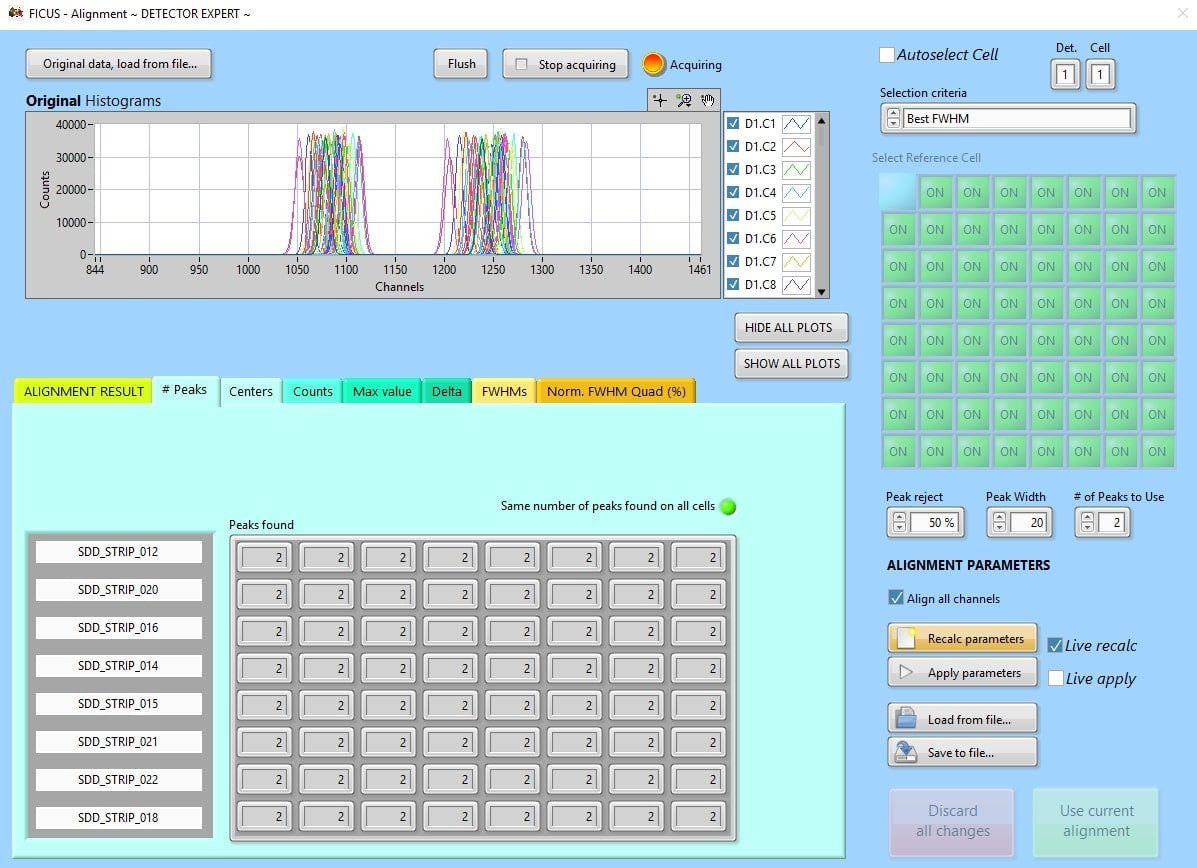
\includegraphics[width=.7\textwidth]{Capture24.jpg}} \quad
\caption{The windows of the FICUS Alignment (Peaks).}\label{fig:fig20}
\end{figure}

\clearpage

\begin{figure}[h]
\centering
\subfloat
{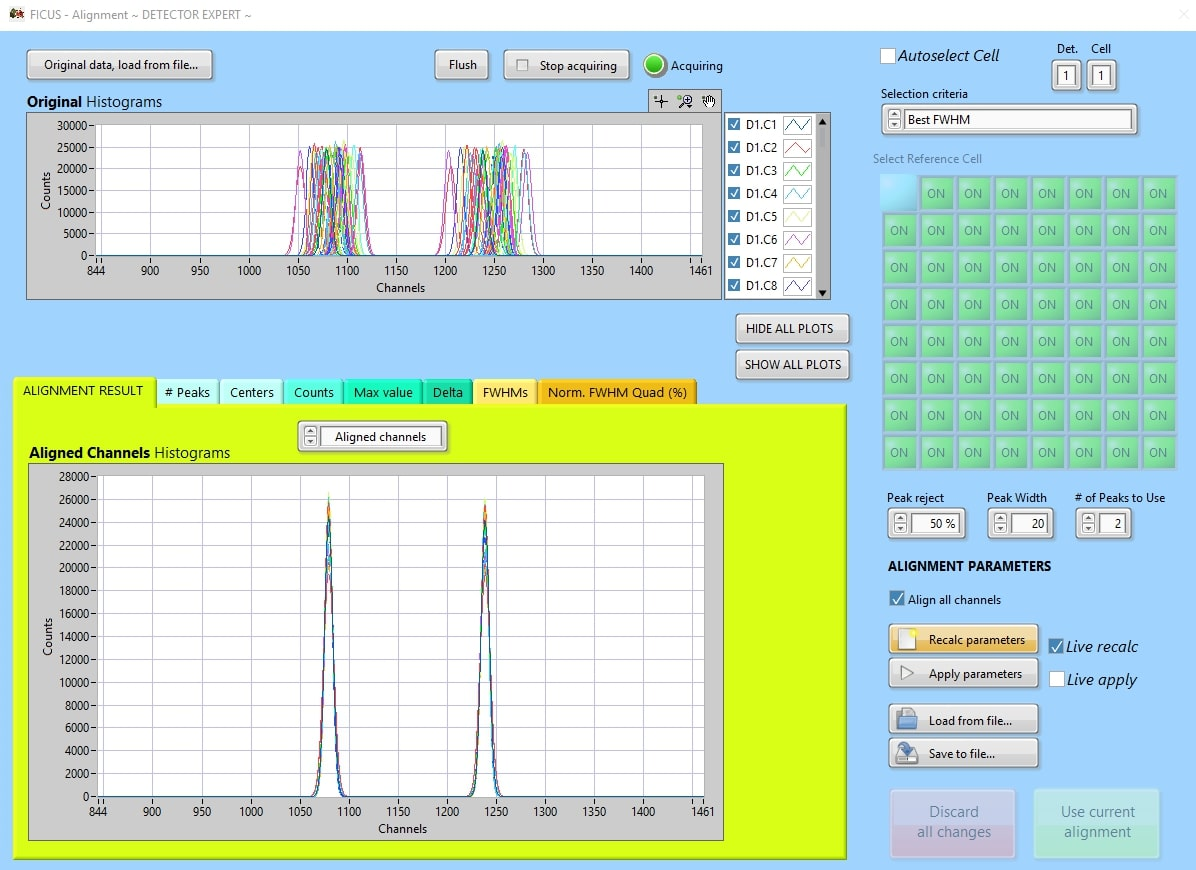
\includegraphics[width=.6\textwidth]{Capture23.jpg}} \\
\subfloat
{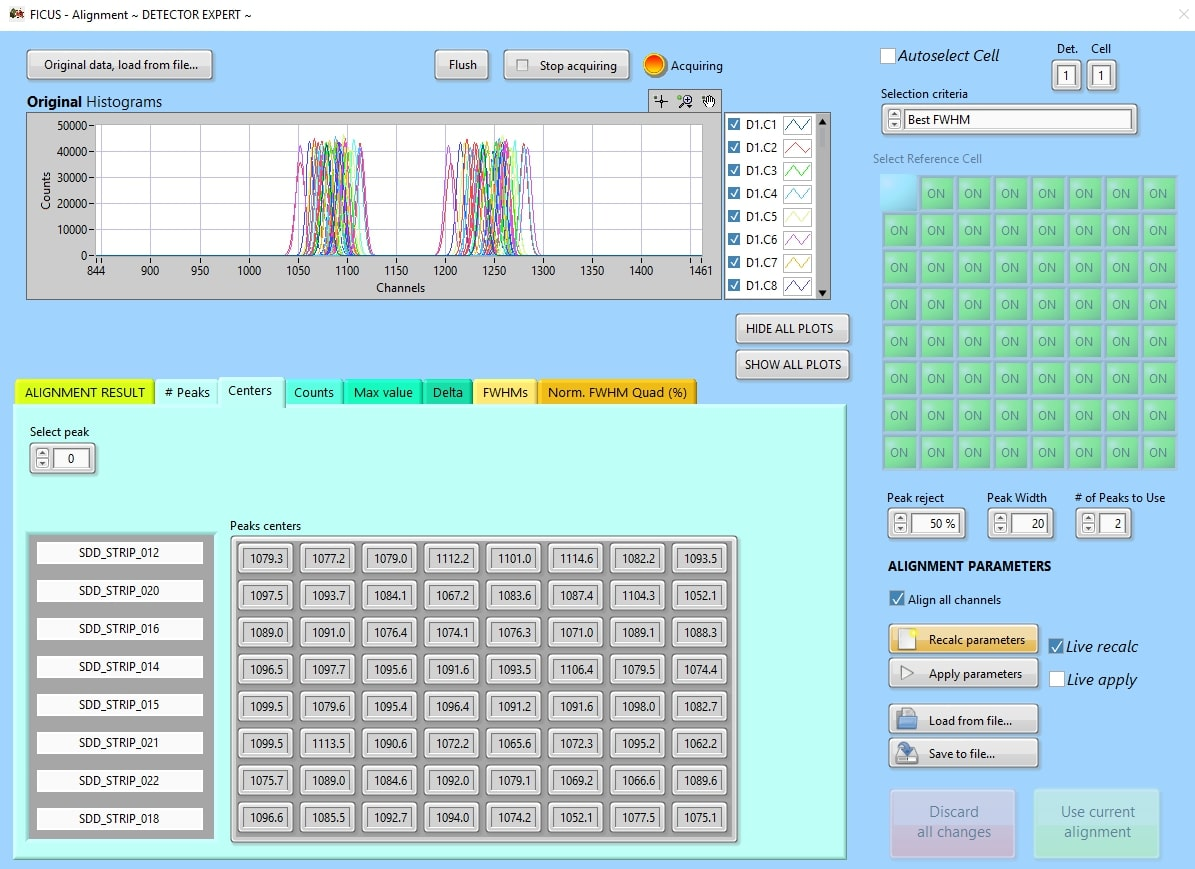
\includegraphics[width=.6\textwidth]{Capture25.jpg}} \\
\subfloat
{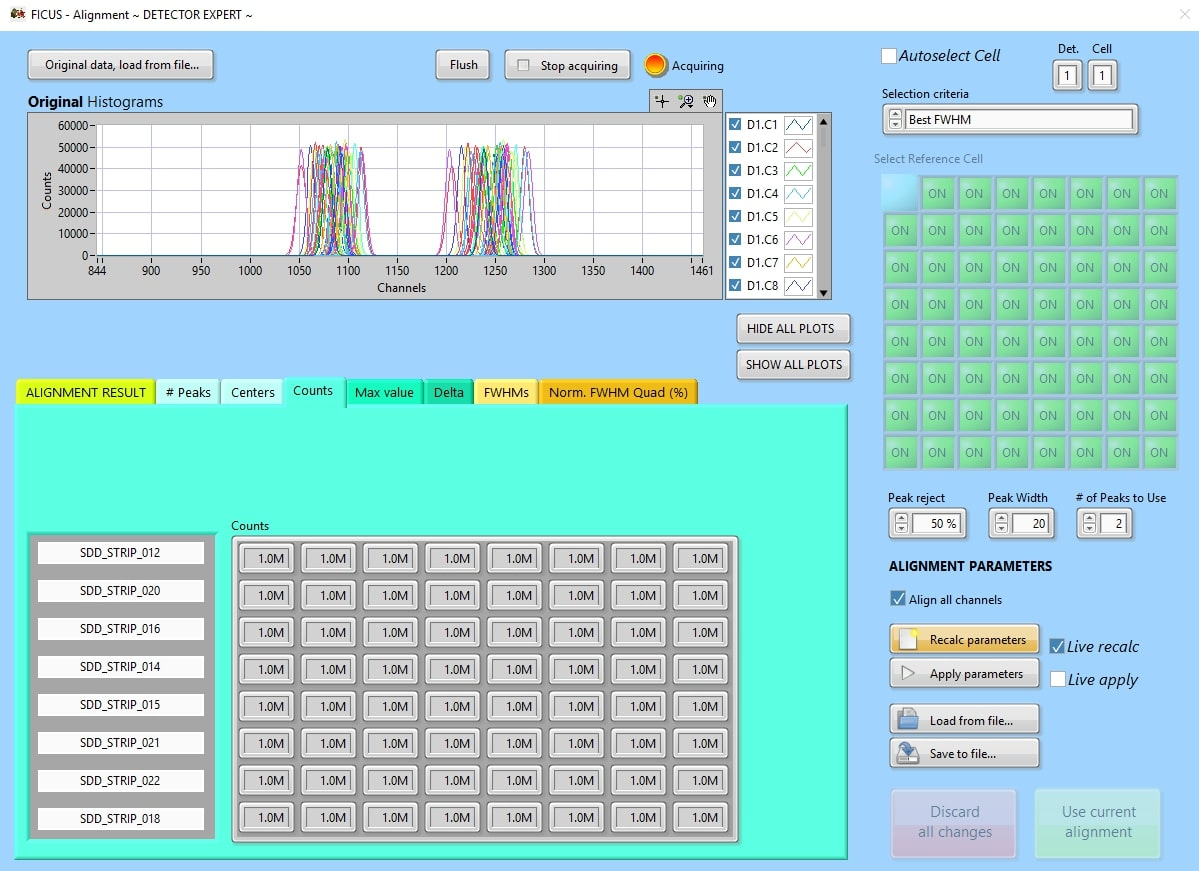
\includegraphics[width=.6\textwidth]{Capture26.jpg}} \\
\caption{The windows of the FICUS Alignment: (\textbf{a}) Alignment Result, (\textbf{b}), Centers, (\textbf{c}) Counts.}\label{fig:fig21}
\end{figure}


\begin{figure}[h]
\centering
\subfloat
{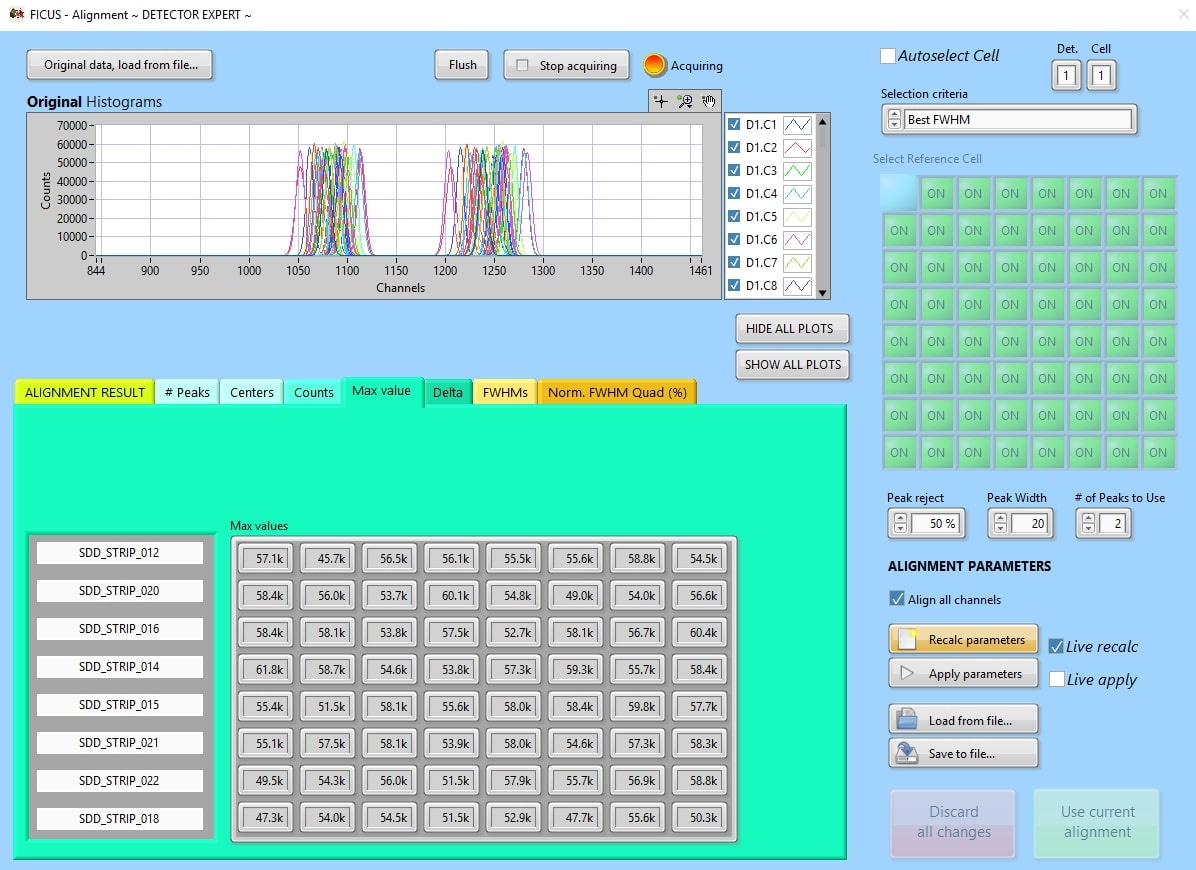
\includegraphics[width=.6\textwidth]{Capture27.jpg}} \\
\subfloat
{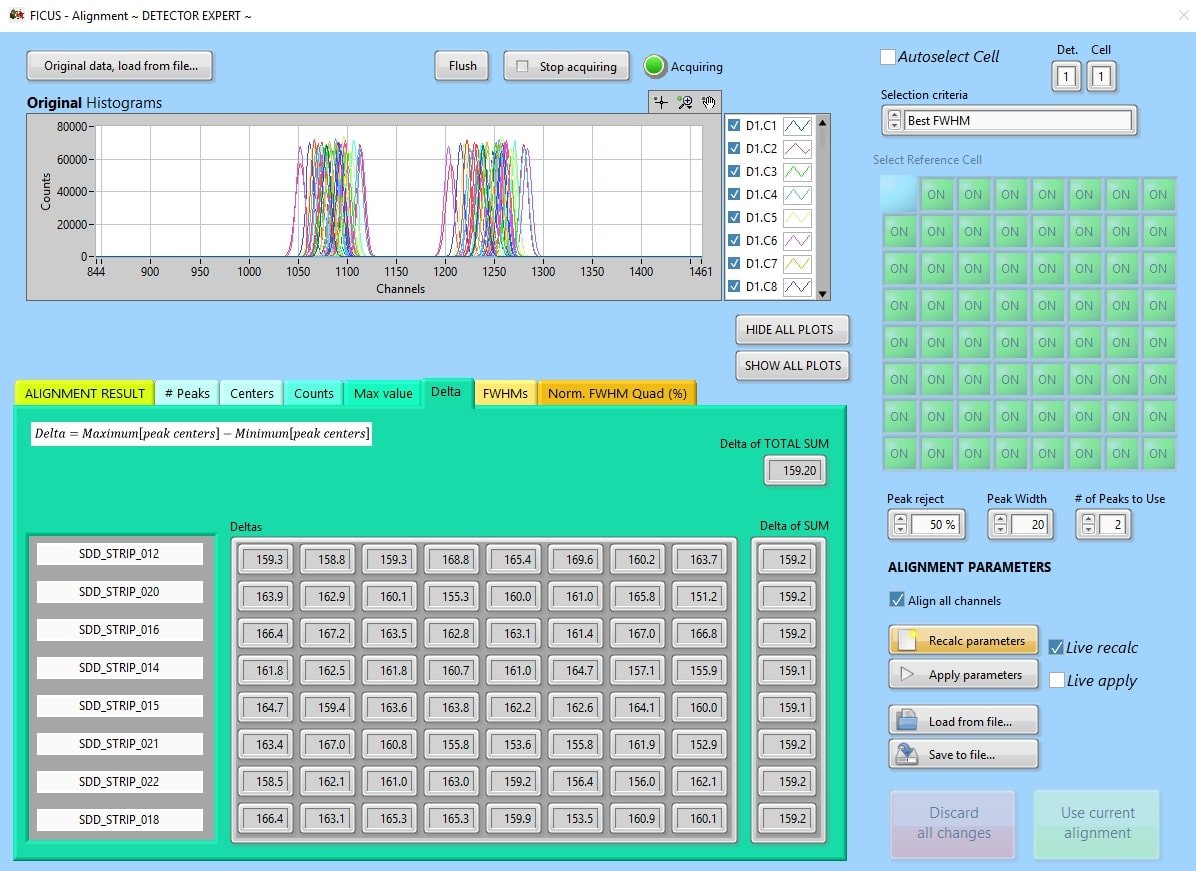
\includegraphics[width=.6\textwidth]{Capture28.jpg}} \\
\subfloat
{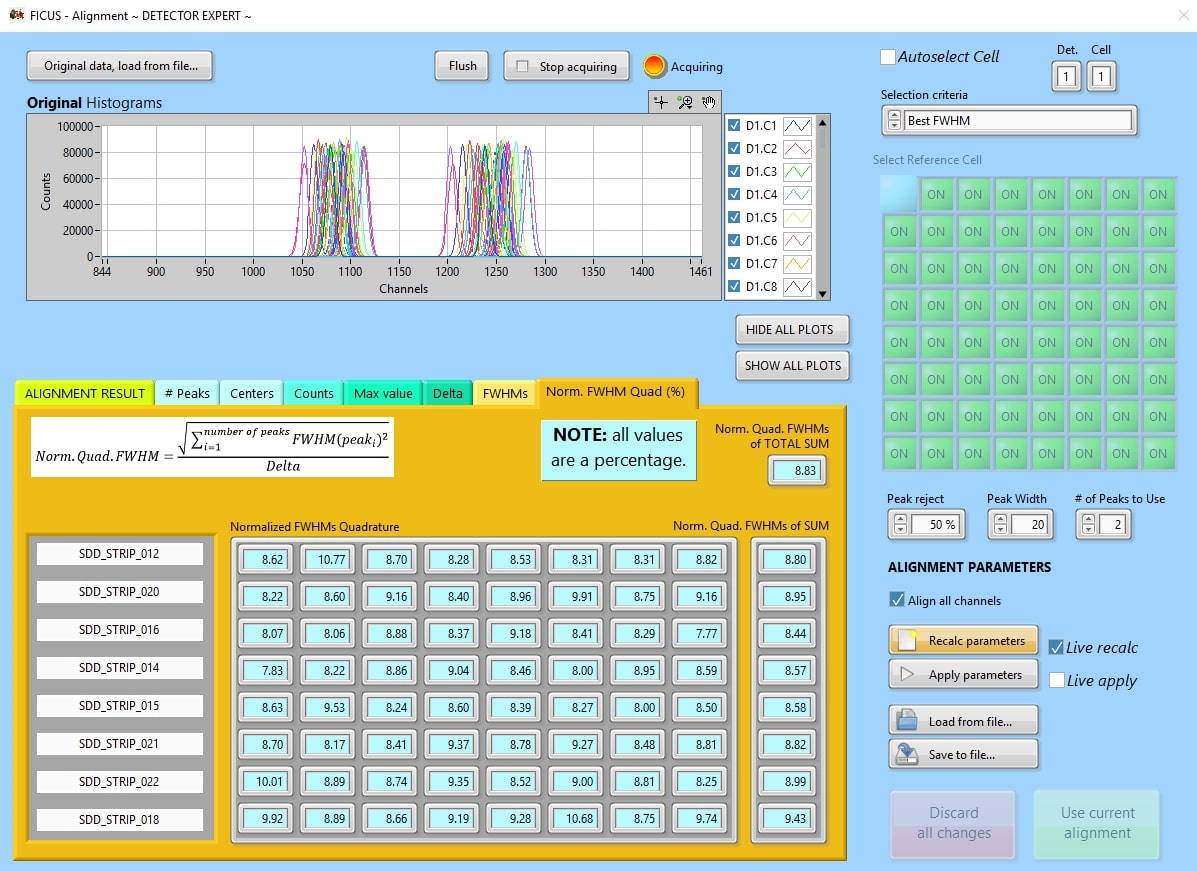
\includegraphics[width=.6\textwidth]{Capture30.jpg}} \\
\caption{The windows of the FICUS Alignment: (\textbf{a}) Max Value, (\textbf{b}), Delta, (\textbf{c}) Norm. FWHM Quad (\%).}\label{fig:fig22}
\end{figure}

\clearpage

To complete the alignment in a short time and effectively it is recommended:
\begin{itemize}
\item to cut through the cursors any signal baseline and escape peak, so as to leave highlighted the peaks on which to do alignment
\item to use alignment parameters such as those in the figure  
\item to wait for the time necessary to have a good signal collection
\item to have the same number of peaks on all channels (and then turn on the light in the \textit{Peaks} box)
\end{itemize}
If it is necessary to leave the alignment procedure without completing it, click on \textit{Discard all changes}.
At the end of the procedure, when you have a good sum signal, (if you want you can save the alignment by clicking on the \textit{Save to file...} button) and  exit the alignment procedure by clicking on \textit{Stop acquiring} and then on \textit{Use current alignment}. This will re-open the acquisition window and the alignment indicator will be coloured green, as shown in Fig. \ref{fig:fig23}.

\begin{figure}[h]
\centering
{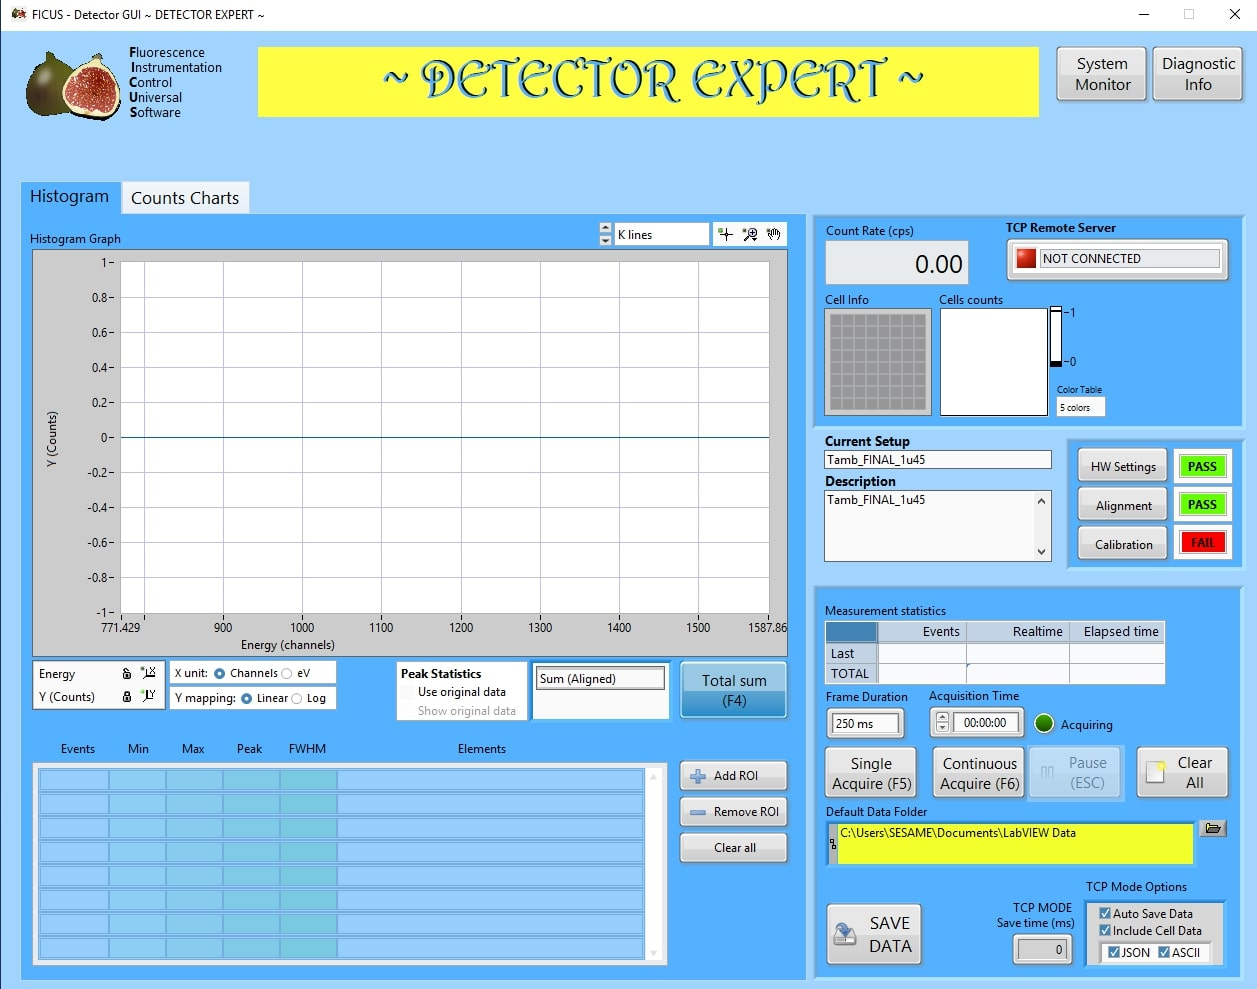
\includegraphics[width=.95\textwidth]{Capture32.jpg}} \quad
\caption{The windows of the FICUS acquisition (Histogram), after Alignment.}\label{fig:fig23}
\end{figure}

Back to the FICUS acquisition window, it is possible to start a measurement by setting the \textit{Frame Duration} and the \textit{Acquisition Time} (in format hh:mm:ss). For a single measurement equal to the duration of the frame click on \textit{Single Acquire (F5)}, for a timed measurement just set the acquisition time and then click on \textit{Continuous Acquire (F6)}. If instead it is wanted to start and stop the measurement manually, it is enough to leave the acquisition time field at zero.

The \textit{Histogram Graph} box shows the accumulated graph of the sum signal [it is also possible to display the signal of the single channels by clicking on \textit{Sum (Aligned)} an additional one will appear in which it is possible to choose which channel to display]. It is possible change manually the ends of the axes or you can zoom by clicking on the magnifying glass symbol (to unlock the ladder just click on the bolt symbol).
It is possible to choose whether to display the Y axis in linear or logarithmic scale, and the X axis in channels or in eV (this is possible only after having performed the calibration procedure).

\begin{figure}[h!]
\centering
{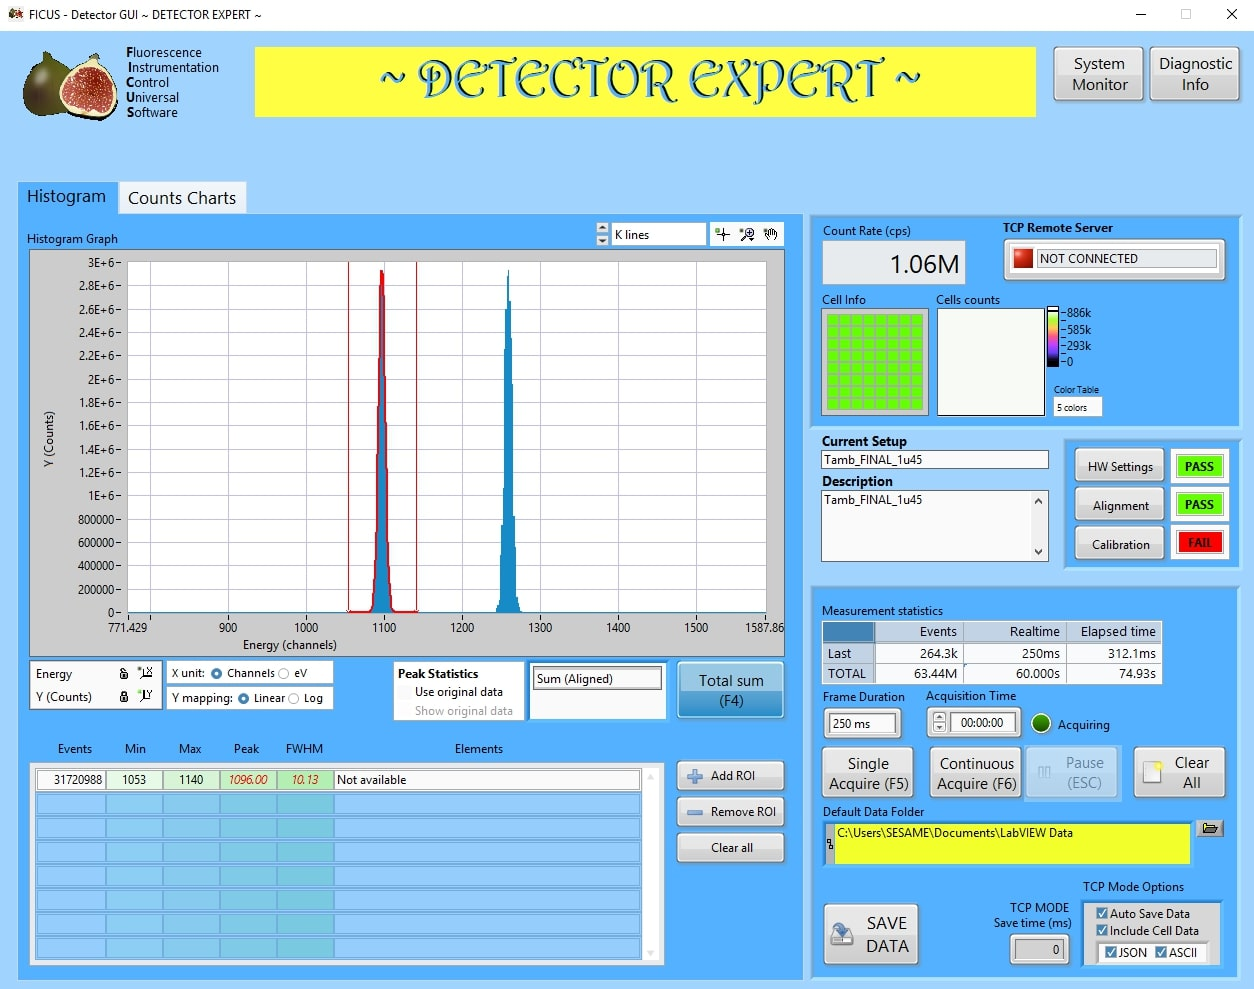
\includegraphics[width=.95\textwidth]{Capture31.jpg}} \quad
\caption{The windows of the FICUS acquisition (Histogram), after the measurement by one minute with VTEST and Double VTEST.}\label{fig:fig24}
\end{figure}

During or after the acquisition it is possible to select Regions Of Interest (ROI) clicking on \textit{Add ROI} and by positioning the sliders manually; up to 20 different ROIs can be selected (there are 4 colours and they repeat cyclically with no choice). 
The table below shows the data of each ROI: \textit{Events}, \textit{Min} position, \textit{Max} position, \textit{Peak} position, and an estimate of the \textit{FWHM} (is calculated as the width at half height considering the intersections of the sliders with the signal). 
If the calibration procedure has been performed, when eV is selected as the X unit, the ROI data also changes the unit of measurement.
The ROI can be removed individually by clicking on \textit{Remove ROI} and selecting the one to be deleted, or all by clicking on \textit{Clear all}.

After stopping or ending the acquisition, it is possible to perform the calibration: clicking on \textit{Calibration} opens the window dedicated to it. \textbf{FICUS Calibration window} appears as in Fig.  \ref{fig:fig25}: the accumulated signal is visible and you can zoom in using the zoom button.
A previously saved calibration file can be loaded (by clicking on \textit{Load from file...}) or a new calibration can be performed. To do this it is necessary to click on \textit{New point...} (to select a point on the x-axis) or on \textit{New region...} (to select the region of the peak we are interested in using cursors, search for the maximum); in the window that appears, write the name of the element corresponding to the centre of the peak and then the corresponding energy.
Repeat the procedure for all peaks you want to identify. If it is necessary to delete one or all of the points inserted, it is possible to do so by clicking on \textit{Delete Calibration Item...} or \textit{Delete All Calibration Items}. To exit without saving or applying the calibration click on \textit{Ignore Change}. When it is considered sufficient, (you can save the calibration by clicking on \textit{Save to file...} and select the name of the file) it is possible to apply the calibration by clicking on \textit{Use This Calibration}. This will re-open the acquisition window and the calibration indicator will be coloured green, as shown in Fig. \ref{fig:fig26}.

\begin{figure}[h!]
\centering
{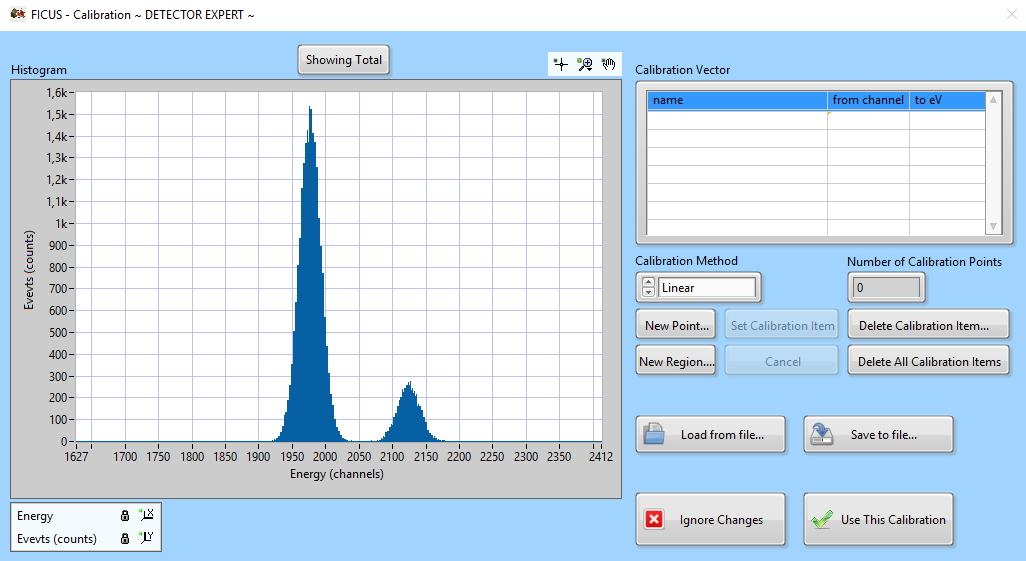
\includegraphics[width=.7\textwidth]{Cattura63.jpg}} \quad
\caption{The windows of the FICUS Calibration.}\label{fig:fig25}
\end{figure}

Instead of the histogram, it is possible to display the \textit{Counts Chart} to monitor the number of total counts and ROI counts [Fig. \ref{fig:fig26}].

\begin{figure}[h]
\centering
{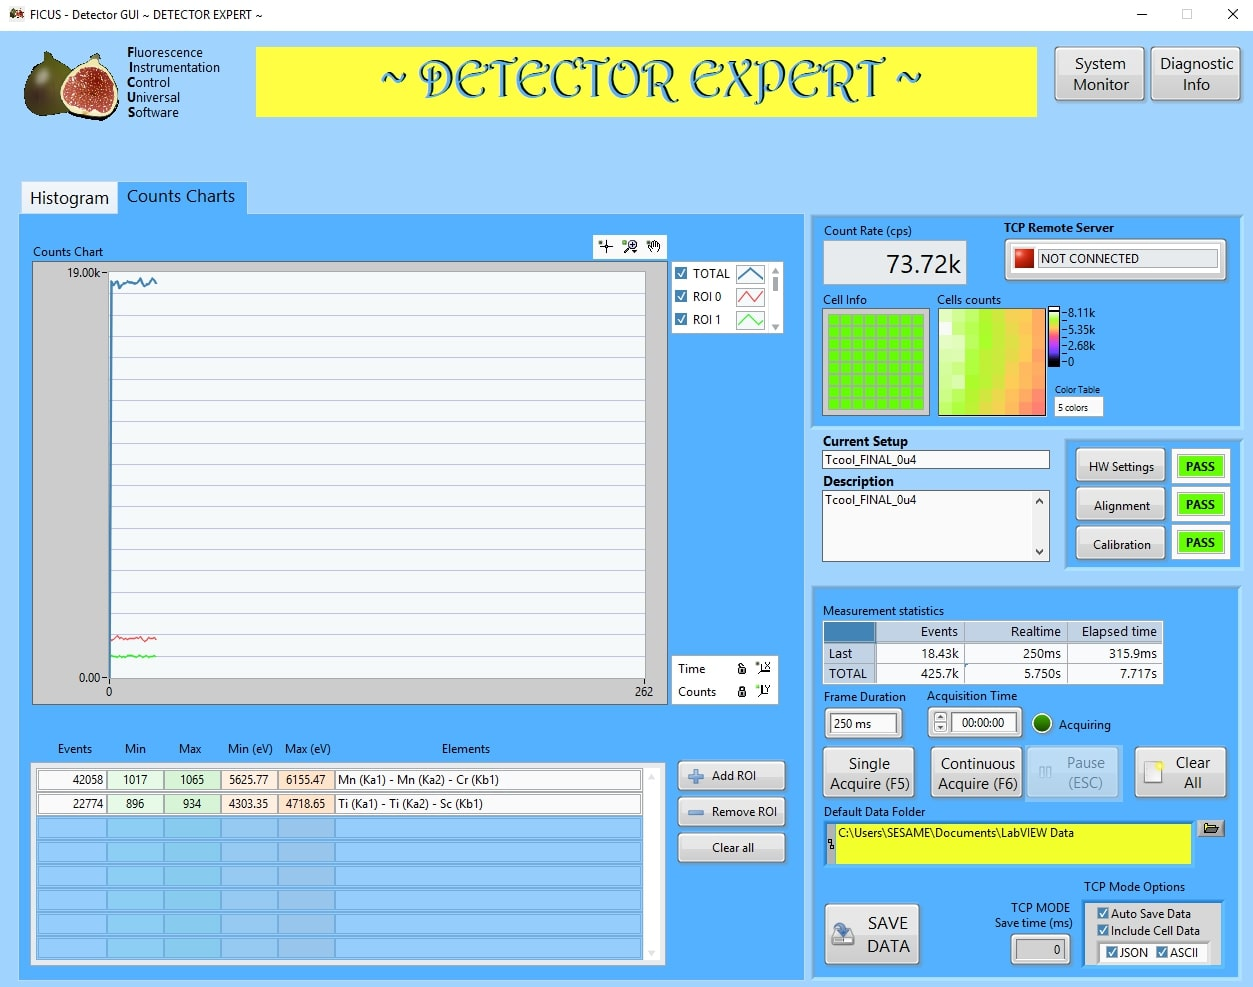
\includegraphics[width=.8\textwidth]{Capture44.jpg}} \quad
\caption{The windows of the FICUS acquisition (Counts Charts), after Alignment and Calibration.}\label{fig:fig26}
\end{figure}

To save the acquired data and the information related to them, just click on \textit{SAVE DATA}, select the saving folder and indicate the name of the file.

To delete the acquisition data, and be ready to start with a new acquisition (continuing to work with the same alignment and calibration) just click on \textit{Clear All}.

\textbf{To switch off the system, carefully follow the switch-off procedure described in the section \textit{Instructions for switching} on on page \pageref{spegnimento}}. 

To close the FICUS software, from the acquisition window click on the \textit{X}, the FICUS control window will appear [Fig. \ref{fig:fig29} (a)]. Click on \textit{Disconnect}, a message will open to confirm disconnecting the detector, press \textit{OK}, as shown in Fig. \ref{fig:fig29} (b). To close the software click on \textit{Quit}, a confirmation message will open, press \textit{OK}, as shown in Fig. \ref{fig:fig29} (c).

\begin{figure}[h]
\centering
\subfloat
{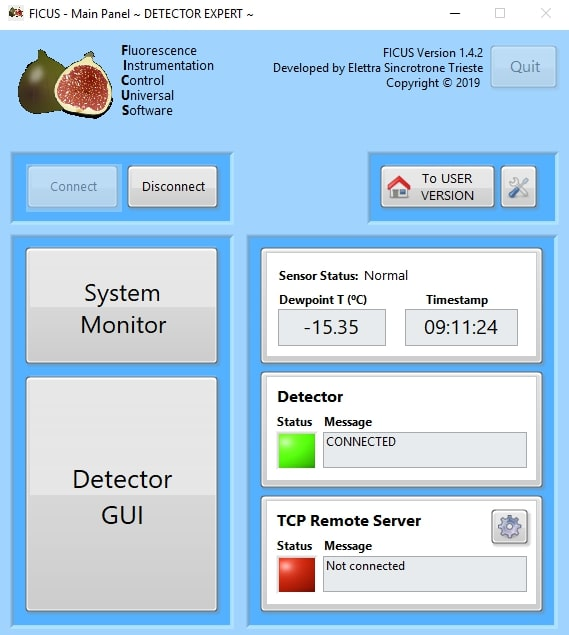
\includegraphics[width=.4\textwidth]{Capture5.jpg}} \\
\subfloat
{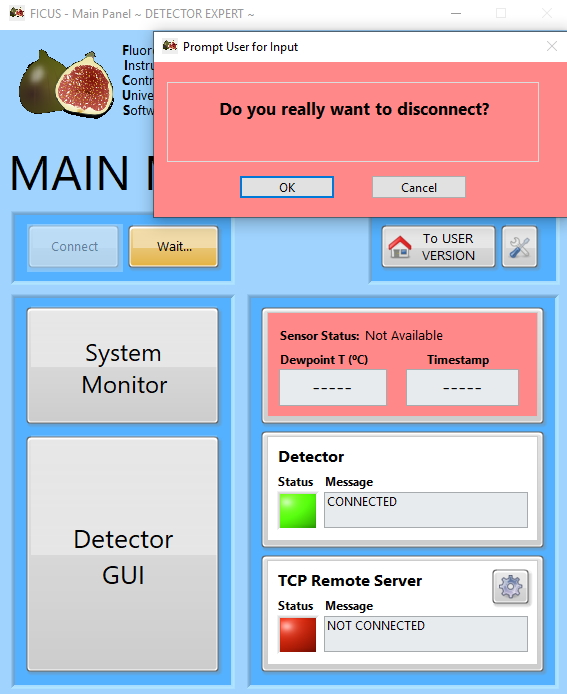
\includegraphics[width=.4\textwidth]{Cattura65.jpg}}  \quad
\subfloat
{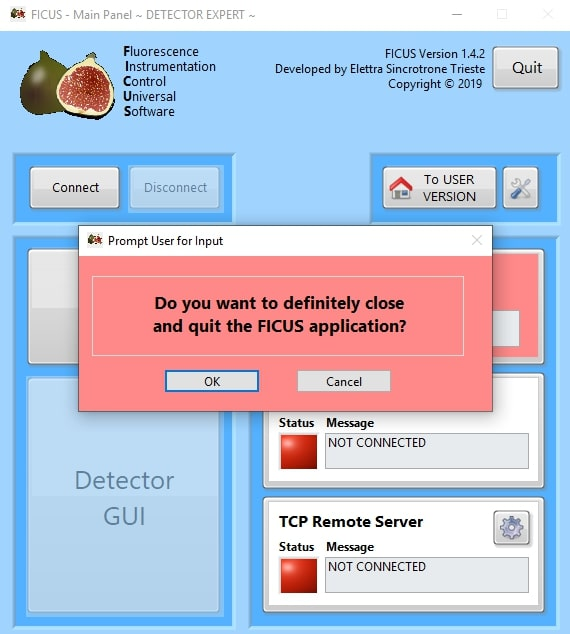
\includegraphics[width=.4\textwidth]{Capture62.jpg}} \\
\caption{The FICUS control window (\textbf{a}) Connected, (\textbf{b}) With the message requesting confirmation to disconnect, (\textbf{c}) Disconnected and with the message requesting confirmation that the program has been closed.}\label{fig:fig29}
\end{figure}

\clearpage

\section{Guide for Beamline Staff}

Before starting any activity, please take a look at the \textbf{Safety warnings for using the SESAME-XAFS Detector System}, on page \pageref{accensione}, and the \textbf{Instructions for switching on/off}, respectively on page \pageref{accensione} and \pageref{spegnimento}.

This version of the software is recommended for the beamline staff in order to optimize the system settings for the planned measurements.

To pass from the FICUS software User version to the Beamline Staff version it is necessary to have the access codes.

Only the FICUS software Beamline Staff version can connect the detectors

















































\clearpage

\section{Guide for User}

Before starting any activity, please take a look at the \textbf{Safety warnings for using the SESAME-XAFS Detector System}, on page \pageref{accensione}, and the \textbf{Instructions for switching on/off}, respectively on page \pageref{accensione} and \pageref{spegnimento}.

This version of the software is useful for the users in order to realize the planned measurements.

Only the FICUS software Beamline Staff version can connect the detectors










































\clearpage

\section{Safety warnings for using the SESAME-XAFS Detector System} \label{sicurezza}
To use the SESAME-XAFS detector system correctly and avoid damaging the measuring system, you must carefully follow the on/off instructions and the software user's guide.
It's very important:
\begin{itemize}
    \item Never switch the HV power supply off and/or on suddenly: it is important gradually increase or decrease the voltage
    \item Never switch the Peltier cells power supply off and/or on suddenly: it is important gradually increase or decrease the voltage
    \item  If the ambient and system temperatures change, it may be necessary to repeat the procedure for loading the appropriate settings, aligning the cells and calibrating the detector
    \item Make sure that the holes for the nitrogen/dry air vent are not obstructed
    \item Make sure that when the flushing is switched on (with appropriate flow rate) the window just swells up
\end{itemize}

    \subsection{Instructions for switching on} \label{accensione}
  It is very important to follow the switch-on procedure following the steps in order and precisely.
    
    \begin{itemize}
        \item Turn on the PC
        \item Start flushing nitrogen / dry air [maximum flow rate of 2 liter/minute]
        \item Turn on the power supply of the dew point temperature sensor [ch3 - analog power supply]
        \item Launch FICUS software
        \item Check that the dew point temperature is below \SI{16}{\celsius} 
            \begin{itemize}
                \item Only if it is so, activate temperature stabilization and turn on the chiller set to \SI{18}{\celsius} 
                \item If it is not so, wait for the dew point temperature to drop below this value thanks to the flushing
            \end{itemize}
        \item Switch on the digital power supply [all ch1, ch2, ch3, ch4 together]
        \item Switch on the analog power supply [ch1 and ch2 of analog power supply]
        \item From FICUS software connect the detector system
        \item From FICUS software load the appropriate settings according to the condition and temperature of use (possible choice of 8 global setups)
        \item Switch on the HV power supply (setting recall mode1), gradually increase the voltage from 0 V to 60 V on ch1 and then from 0 V to 60 V on ch2
        \item Wait about 5 minutes for the temperature of the detector to stabilize
        \item Proceed with cell alignment (o load a previously saved alignment setting)
        \item Now it is possible activate measurement
        \item After stop the measurement, proceed with the calibration of the detector system (o load a previously saved calibration)
        \item If you want work in cooling mode (to lower cell temperature), start the instruction for cooling mode
        \end{itemize}

	
    \subsection{Instructions for switching off} \label{spegnimento}
      It is very important to follow the switch-off procedure following the steps in order and precisely.
    
    \begin{itemize}
        \item Gradually decrease the voltage from 60 V to 0 V on ch2 and then from 60 V to 0 V on ch1, and after switch off the HV power supply 
        \item In FICUS close the acquisition window and disconnect the detector
        \item Switch off analog power [ch1 and ch2 analog power]
        \item Switch off the digital power supply [all ch1, ch2, ch3, ch4 together]
        \item Turn off FICUS software
        \item Turn off flushing nitrogen / dry air 
        \item For long detector shutdown or if it is necessary, switch off the dew point temperature meter power supply [ch3 - analog power supply] and turn off the chiller
        \item Turn off the PC
    \end{itemize}
    
    \subsection{Instructions for cooling mode} 
     \begin{itemize}
        \item Before starting the Peltier cell ignition procedure, check that the dew point temperature is below \SI{-12}{\celsius}
        \item Never switch the Peltier cells power supply off and/or on suddenly: it is important gradually increase or decrease the voltage
        \item Switching on and off of the Peltier cells have to be gradual: power supply for 0.1 V steps every 2 min (maximum voltage 2 V)
        \item When the supply voltage of Peltier cells is 2 V, wait at least 5 minutes for the temperature of the detector to stabilize
        \item When the cooling mode is activated, remember to load the appropriate global settings [Tcool] in FICUS
    \end{itemize}   
    
\section{Troubleshooting}
In this section some possible errors or problems that may occur, along with how to fix them. \textbf{If the problem is not listed, please contact the ReDSoX Collaboration.}

\begin{itemize}
    \item \textbf{TCP-IP or/and FPGA tests aren't successful for one or more strips} - There may be problems with FPGAs or communication boards. Try turning off the system (following the switch-off instructions) and, following the switch-on instructions, try switch it on again from the beginning.
    \item \textbf{One or more channels pass from active and functioning to non-active for no apparent reason } - There may be problems with FPGAs or communication boards. Try turning off the system (following the switch-off instructions) and, following the switch-on instructions, try switch it on again from the beginning. If the problem is not solved, try again the shutdown procedure by exiting the software and restarting the PC. And then reactivate everything by following the switch-on procedure. If the problem is not solved even in this way, contact the ReDSoX Collaboration.
    \item \textbf{One or more temperature values have abnormal and different values than normal, or are equal to zero} - Check that the chiller is on and set to the correct value. Try turning off the system (following the switch-off instructions) and, following the switch-on instructions, after a few minutes, try switch it on again from the beginning.
    \item \textbf{The value of the dew point temperature does not decrease with the nitrogen / dry air fluxing} - Check that the nitrogen/dry air flow is active and at the values recommended by the manual. Check that the window is intact and well stretched.
    \item \textbf{The sum signal of the channels appears deformed} - Try realigning the channels.
    \item \textbf{One or more power supplies do not turn on} - Check the correct connection of the power supply to the electric grid.
\end{itemize}

\section{Information \& Contact - ReDSoX Collaboration}
        The FICUS software was developed by Elettra Sincrotrone Trieste.
        
        This software manual (about FICUS 1.4.2.0 and FICUS 1.4.2.1) has been prepared by the testers of the detector system (detector expert) of INFN-Ts.
        
        The SESAME-XAFS detector system implementation is managed by the Istituto Nazionale di Fisica Nucleare (INFN) in collaboration with Elettra Sincrotrone Trieste, within the ReDSoX (Research Drift detectors for Soft X-ray) collaboration by INFN and Elettra (and other entities listed below in alphabetical order) thanks to ad hoc financing from the Ministry of Education, University and Research (MIUR).
	
        In particular, this work has been made within the ReDSoX-2 INFN research project, supported with the contribution of the Italian Ministry of Education, University and Research within the EUROFEL Project and FBK-INFN agreement 2015-03-06.
	


\end{document}

